\chapter{AI Powered Society}

\begin{center}
{\large\uppercase{Rajendra K. Bera}}
%\footnote{Chief Mentor, email: rajendrabera@yahoo.com. Communicating author. The views expressed are those currently held by the author.}

\thispagestyle{empty}

\vskip -6pt

Chief Mentor, Acadinnet Education Services India Pvt.
\end{center}
\vskip 1.5cm

\noindent\makebox[\textwidth]{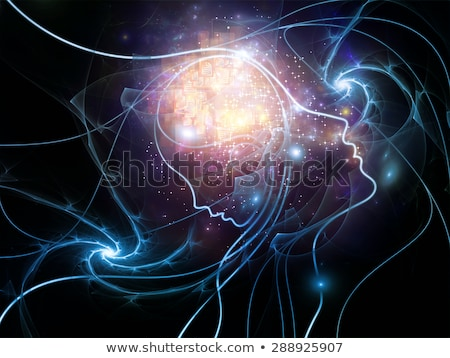
\includegraphics[width=1.05\paperwidth,height=17cm]{src/Figures/AI_powered_society.jpg}}

\newpage

\begin{multicols}{2}
\section*{Abstract}

To understand the post-industrial world of the millennials and the challenges and opportunities it presents is yet another chapter in the evolution of \textit{Homo sapiens}. It will force humanity to reassess the meaning of life, its place and significance in the Universe, and above all its ability to survive in a world that includes its own creative creation - the super-intelligent, human-machine hybrid - the humanoid. The role of natural humans and humanity's faith in spirituality if humanoids take charge will undergo a sea-change. The millennials' ability to adapt to the new world by competing against the humanoids will face severe limitations and may even lead to \textit{Homo sapiens} becoming an endangered species within a century. A biological evolution of intelligent life is waiting to happen, triggered by the \textit{Homo sapiens’} curiosity-driven quest to understand the Universe within a rational, axiomatized framework.

\smallskip
\noindent
{\it\bfseries Keywords:}~Artificial intelligence, post-industrial economy, millennials, rationalism.\\[-21pt]

\section{Introduction}

Recent advances in artificial intelligence (AI) and biotechnology are nothing short of sensational in terms of the conceptual barriers they have overcome. In the last few years they have garnered a list of achievements and synergistic integration that clearly indicate that \textit{Homo sapiens} are in for an unprecedented upheaval in their life--the loss of their vaunted intellectual supremacy on Earth and the rising role of humanoids in human affairs. This change will likely happen within a century if Kurzweil's predictions about the future of AI come true (given his track record, it most likely will). Kurzweil, the author of \textit{The Singularity is Near}\footnote{Kurzweil (2005).} predicts: “By 2029, computers will have human-level intelligence.”\footnote{Fox News (20170316).} He also says the future will provide opportunities of unparalleled human-machine synthesis. In a communication to Futurism, Kurzweil said:
\begin{quote}
2029 is the consistent date I have predicted for when an AI will pass a valid Turing test and therefore achieve human levels of intelligence. I have set the date 2045 for the `Singularity' which is when we will multiply our effective intelligence a billion-fold by merging with the intelligence we have created.\footnote{Galeon \& Reedy (2017). “Of his 147 predictions since the 1990s, Kurzweil claims an 86 percent accuracy rate.”}
\end{quote}

To this we add an observation by Richard Ogle in his book, \textit{Smart World:}
\begin{quote}
[I]n making sense of the world, acting intelligently, and solving problems creatively, we do not rely solely on our mind's internal resources. Instead, we constantly have recourse to a vast array of culturally and socially embodied \textit{idea-spaces} that populate the extended mind. These spaces ...  are rich with embedded intelligence that we have progressively offloaded into our physical, social, and cultural environment for the sake of simplifying the burden on our own minds of rendering the world intelligible. Sometimes the space of ideas thinks for us.\footnote{Ogle (2007).}
\end{quote}

This smart world also faces unprecedented demographic changes due to variations in mortality, life expectancy, and a youthful population in countries where fertility is high. Overcrowding on Earth is a recent phenomenon. In the next three or four decades, the overall population of the more developed countries is likely to stagnate at about 1.3 billion (see Fig.~1.1). Their population is ageing and would decline but for migration. The populations of Germany, Italy, Japan, and several states of the former Soviet Union that broke away are also expected to decline by 2050.\footnote{See, e.g., UNPF (2017).} The world's flexibility to cope with such unprecedented socio-economic changes is untested. Hence the millennials are expected to face unprecedented challenges and novel opportunities in the future. It will force humanity to reassess the meaning of life, its place and significance in the Universe, and above all its ability to survive in a world that includes its own creative creation - the super-intelligent, human-machine hybrid - the humanoid. The role of natural humans (the \textit{Homo sapiens}) and humanity's faith in spirituality if humanoids take charge will undergo a sea-change. Humanity's ability to adapt to the new world by competing against humanoids will be severely tested and may even lead to the \textit{Homo sapiens} becoming an endangered species within a century. A biological evolution of intelligent life is waiting to happen, triggered by the \textit{Homo sapiens'} quest to understand the Universe not according to the scriptures but according to science.\\[-22pt]

\section{Life on Earth}

\vskip -4pt

{\parfillskip=0pt
Life on Earth began some 3.8 billion years ago with single-celled prokaryotic cells, such as bacteria, evolving to multi-cellular life over a billion years. It\par}
\end{multicols}

\begin{figure}[H]
\centering

\includegraphics[scale=1.15]{src/Figures/chap1/1.eps}
\end{figure}

\begin{multicols}{2}

\noindent
is only in the last 570 million years that life forms we are familiar with began to evolve, starting with arthropods, followed by fish 530 million years ago (Mya), land plants 475 Mya, and forests 385 Mya. Mammals evolved around 200 Mya, and \textit{Homo sapiens} (the species to which we humans belong evolved from \textit{Homo erectus})\footnote{Davis (2018). \textit{Homo erectus} had bodies similar to modern humans, could make tools, and were possibly the first to cook. They may have been mariners and possibly had a language. They first appeared in Africa more than 1.8 mya and wre perhaps the first archaic human species to leave the continent.} arose only a mere 300,000 years ago.\footnote{BBC (2018). \textit{See also:} SNMNH (2018b).} Up until 2.4 billion years ago, there was no oxygen in the air. There is still much to learn about the \textit{Homo sapiens}.\footnote{Maropeng (20100409). \textit{See also:} Berger (2015); Berger \& Hawks (2017); Greshko (2017) (“After adding \textit{Homo naledi} to the human family tree, researchers reveal that the species is younger than it seems. ... Lee Berger--provides an age range for the [fossil] remains first reported in 2015: between 236,000 and 335,000 years old.”); Barras (2017a) (“The past 15 years have called into question every assumption about who we are and where we came from. Turns out our evolution is more baffling than we thought.”); Barras (2017b) (“Lee Berger’s stunning discoveries of huge caches of ancient bones are overturning ideas about our origins, but not everyone likes his methods.”).} Their origin is vastly different from what various religions tell us. They were not made by God in His own image; they evolved to their present image and they are still evolving in unknown ways. One day, the \textit{Homo sapiens} will become the ancestor species of one or more species. No religion has ever alluded to that.

On the biological front, Darwin's theory\footnote{Darwin (1859).} of evolution of life was a remarkable eye-opener. He posited that all life is related and that it descended from a common ancestor: the birds and the bananas, the fishes and the flowers, the animals and the \textit{Homo sapiens, etc.} It presumes life developed from non-life and that complex creatures evolve from less complex ancestors naturally and over time through a random process of adaptation via “descent with modification” in which random genetic mutations occur within an organism's genetic code; the beneficial mutations that aid an organism to survive are  thus passed on to the next generation while the weaker organisms die and are eliminated from breeding--a process known as “natural selection” or survival of the fittest in a given environment. Over time, enough beneficial mutations accumulate to trigger a phase transition and an entirely different organism (not just a variation of the original) comes into existence. The supporting evidence for Darwin's theory of evolution comes from morphological similarity among organisms (suggesting shared descent), and that living species are similar to recent related fossils. The fossil record is good and large enough for us to see relatives of clearly different species in it.\footnote{See, \textit{e.g.,} Dawkins (2010).}

Evolutionary biology by itself does not necessarily imply that God does not exist. But it admits the plausible view: “If God does exist, however, existing is about the only thing He has ever done. God is permanently unemployed, if, in the entire history of life, impersonal material forces were capable of doing the whole job and did do it. So if one attempts to hold a view of God as creator, it is a very attenuated view and one which tends to fade away into unreality.”\footnote{Provine \& Johnson (1995).}  There is still much to learn about the nature of biological diversity and its complexity. We do not yet know how genetic information, as encoded in the DNA, came into existence to start life out of single-celled predecessors. That this is what happened millions of years ago is a reasonable scientific conjecture not yet refuted. Man learnt thousands of years ago how to accelerate the natural evolution process through selective breeding, \textit{i.e.,} by reducing randomness in the selection process, say, dogs with specific characteristics (\textit{e.g.,} size, body color, hair type, demeanor, \textit{etc.}) or plants modified to taste, made sturdier, etc., within a few thousand years rather than hundreds of millions of years that natural selection would take. Early human-engineered breeding practices have now advanced to an extent where we can clone living organisms and directly modify a living or dead organism's DNA or even \textit{ab initio} design DNA to create new organisms in the lab. We call it biotechnology, the core of which is genetic engineering. Creation of living matter is no longer a mystery, but how non-living matter gets turned into life and vice-versa is still a mystery.

Man's association with dogs goes back to some 10,000 to 30,000 years ago. It is generally believed that “all dogs, from low-slung corgis to towering mastiffs, are the tame descendants of wild ancestral wolves.”\footnote{Yong (2016).} Wolves, living in and around human surroundings, grew tamer with each generation until they became domesticated permanent companions. Dogs have cross-bred so often with wolves and each other that we have a great variety of them. The process itself indicates that dog domestication may have happened several times spread over different geographies and times. Some day, molecular biologists may tell us how ancient canines relate to each other and to modern pooches. The domestication of the grey wolf into dogs, man's reputed best friend, happened long before the Industrial Revolution (1760-1840), before literature and mathematics, and before bronze, iron, and agriculture. This ancient partnership between man and animal entwined the fate of the two species. “The wolves changed in body and temperament. Their skulls, teeth, and paws shrank. Their ears flopped. They gained a docile disposition, becoming both less frightening and less fearful. They learned to read the complex expressions that ripple across human faces. They turned into dogs.”\footnote{Yong (2016).}

The domesticated dog is an outstanding example that man is the important factor on Earth in changing the environment. It is he who could domesticate a wild species through genetic breeding in a very small fraction of the time that Nature would have required. And now that man has learnt the secret of creating new species in a lab, the time is not too far when he would be doing it on a mass scale.

Interestingly, no religion talks about either the bacteria or the dinosaur or the evolution of man from the great apes. The dog does get a mention. Till an explosion in scientific knowledge occurred and directly began to affect the structure of human societies through new schemes of division of labor and its institutions, religion had a stranglehold on man that transcended the powers of human rulers. Since the 20$^{\rm{ th}}$ century, religion's power over educated man has begun to erode with increasing momentum. The simple dilemma of the millennials is: Should they enjoy and explore life on Earth or secure a place in heaven by servilely appeasing an unseen, undescribable God who communicates with men through messengers claiming to carry revealed messages whose contents are increasingly at variance from science. Science is progressive and open to correction, religion is regressive and dogmatic.

Religions are oblivious of millions of species that once existed on Earth and have since vanished and millions that will emerge on Earth in the future.\footnote{\textit{See, e.g.,} Han (2013). \textit{See also:} CBD (), WWF Global (2017), Pearce (2015).} Indeed, we have no idea how and to what \textit{Homo sapiens} will become ancestors to. For example, geology tells us how plate tectonics has changed the location of continents through movements of plates on the Earth's surface. This has helped scientists correlate in spatial-temporal terms the geographical distribution of animals and plants, both living and fossil, with plate movements. This is amazing evidence for evolution by shared descent. It is generally estimated that there were about fifty thousand species of vertebrates just 65-70 million years ago, to the end of the Cretaceous. Of those, fewer than twenty gave rise to some one hundred thousand species of vertebrates that exist now. The rest became extinct.\footnote{Provine \& Johnson (1995).}  One wonders why God let them all die instead of letting them live in harmony.

Life on earth began nearly four billion years ago. In another billion years life will become extinct because the Sun's brightness is increasing nearly 10 percent per billion years, enough to extinguish life on Earth by incineration.\footnote{Starr (2018).} In another 10 billion years from now, the Sun too will die in a spectacular display of fireworks. It does not matter if we devoutly and religiously believe the Sun to be a god or not.\footnote{With the death of the Sun, Hinduism, allegedly the oldest of religions, will lose one of its most important gods. Of course, his worshippers would have died long ago by then.} As William Provine says,
\begin{quote}
Let me summarize my views on what modern evolutionary biology tells us loud and clear - and these are basically Darwin's views. There are no gods, no purposes, and no goal-directed forces of any kind. There is no life after death. When I die, I am absolutely certain that I am going to be dead. That's the end of me. There is no ultimate foundation for ethics, no ultimate meaning in life, and no free will for humans, either.\footnote{Provine \& Johnson (1995).}
\end{quote}

This is quite the opposite of what religions preach us, namely, God created life and humans He created separately. Humans and chimpanzees do not share a common ancestor. God gives life after death and He gives us absolute foundation for ethics. He also gives us the ultimate meaning for life and gives us free will to go astray or seek genuine understanding of Him and shoulder responsibility. No reason was ever provided for not creating the perfect man and the perfect universe in the first place. Also, free will gives man the opportunity to act as nastily and irresponsibly as God does, like putting people in hell-like prisons and fanning vindictiveness. There is no Earthly reward for praising God and suffering while doing so. The biologically evolving \textit{Homo sapiens} are indeed a small part of a complex, process; they are not the final goal of evolution. “Think of us all as young leaves on this ancient and gigantic tree of life - connected by invisible branches not just to each other but to our extinct relatives and
our evolutionary ancestors.”\footnote{Chakrabarty (2018).}\\[-22pt]

\section{The evolving \textit{Homo sapiens}}

We, the \textit{Homo sapiens}, have been around for about 300,000 years.\footnote{SNMNH (2018b). \textit{See also} the original papers announcing the discovery in Nature: Hublin, et al. (2017), and Richter, et al. (2017). Prior to these papers, \textit{Homo sapiens} were said to have been around for about 200,000 years.} Records of our civilization date back approximately 6000 years. About 12,000 years ago, after more than 99\% of mankind's life on Earth, man transitioned from being the nomadic hunter-gatherer to a pastoral-agricultural life of rearing animals and sowing seeds. This lasted till about 1500 AD. During this period society structured itself into families; women took care of the household, men earned a livelihood. From about 1500 AD to the later-half of 20$^{\rm th}$ century, an industrial economy developed with increasing growth of industrial activity and mechanization of agriculture. Within five centuries, the economy graduated from using animal power to steam power to fossil fuel power to electrical power. Along with changing sources of power, society too restructured itself into increasingly complex communities--extended families, cities, nations, alliances, institutions, modes of governance, dominions, \textit{etc.}--and economies that ranged from family businesses run locally to multinational corporations operating globally and employing millions of men and women. Women were gradually weaned away from the hearth to the power corridors of corporations, competing with men for power and success in all spheres of life--business, politics, arts, science, \textit{etc.} Since the late 20$^{\rm th}$ century the world began to transform rapidly into a post-industrial economy which expects to power its way to another future using wind, solar, and information power. This, in brief, is the progress of human civilization.\\[-12pt]

\subsection{The hunter-gatherer stage}

In the hunter-gatherer stage, humans and their socio-economic organizations and skills developed at an ultraslow pace consistent with Darwin's theory of evolution by natural selection.\footnote{Darwin (1859). It carries the apt subtitle “On the Preservation of Favoured Races in the Struggle for Life”} In the subtitle of his book, \textit{On the Origin of Species by Means of Natural Selection} (1859), Darwin aptly saw it as the “Preservation of Favoured Races in the Struggle for Life”. The struggle continues. The core hypothesis of the theory is that species with traits that help in adaptation are more likely to survive and reproduce than its peers in a given environment. The role of the human mind would have been negligible in such an evolutionary process. Human population was sparse; space required for survival per inhabitant was about a square mile and demanded a nomadic life involving extraordinary land-intensive activity.\footnote{Bernstein (2004).} Its advanced technology was built around stone to make implements with a sharp edge, a point, or a percussion surface.\\[-12pt]

\subsection{The agricultural stage}

In comparison, in a span of mere 12,000 years, in the agricultural stage, the human brain-mind began to flex its neural network and mentally awakened humans began to organize into families and communities with progressively more sophisticated systems of division of labor according to the size of the community and its contextual function. An adaptive civilization emerged from an evolutionary process that took survival of the fittest to the community level:
\begin{quote}
One of the earliest defining human traits, bipedalism – the ability to walk on two legs – evolved over 4 million years ago. Other important human characteristics – such as a large and complex brain, the ability to make and use tools, and the capacity for language – developed more recently. Many advanced traits – including complex symbolic expression, art, and elaborate cultural diversity – emerged mainly during the past 100,000 years.\footnote{SNMNH (2018a).}
\end{quote}
Biological evolution is not about individuals, it is about inherited means of growth and development that enhances the survivability of a population of a given species evolving in a given habitat. The most important characteristic feature of the agriculture stage of human evolution was the emergence of an adaptive brain-brawn feedback system that would continuously monitor and tweak the environment to improve conditions for human survival. Within its limited geographical perimeter, a community freed itself from the terrors of the animal kingdom where Nature is “red in tooth and claw”.\footnote{So was Nature described by the poet Lord Tennyson in \textit{In Memoriam A.H.H. (1849), http://www.online-literature.com/tennyson/718/} before Darwin published his theory about the origin of species in 1859.} For the first time, humans evolved not purely by physical adaptation in an environment but by also mentally adapting to and changing the environment by putting his mind to work in coordination with the rest of his body.

Once the capacity to create and use language and the ability to work with metals (copper, bronze, iron) developed, human civilization evolved rapidly. Communication became the backbone of human civilization to link minds, exchange ideas, govern, intimidate, chastise, reward, entertain, create and commune with gods, and link past and future generations. It invented the rule of law, put its faith in an unseen, omnipresent, omniscient, omnipotent God, nurtured the fine arts, and laid the foundation for logic, mathematics, and physics. The agriculture stage proved to be vastly more productive than the hunter-gatherer stage; it allowed population density to increase to a few hundred per square mile in settlements with greater safety and food security.\footnote{Bernstein (2004).} Farming communities gradually developed groups with specialized roles, \textit{e.g.,} soldier, ruler, and eventually the institution of individual property rights. When individual farmers began owning and cultivating their plots of land, it created a competitive spirit that greatly boosted efficiency and productivity. North and Thomas note: 
\begin{quote}
It is this change in incentive that explains the rapid progress made by mankind in the last 10,000 years in contrast to his slow development during the era as a primitive hunter/gatherer.\footnote{North \& Thomas (1977). The Sveriges Riksbank Prize in Economic Sciences in Memory of Alfred Nobel 1993 was awarded to Robert W. Fogel and Douglass C. North “for having renewed research in economic history by applying economic theory and quantitative methods in order to explain economic and institutional change.”}
\end{quote}

In the agriculture age, the role of the human mind had suddenly increased. The brain and the brawn (scholar and soldier) were competing for supremacy in social status. Human population and sustainable population density per square mile had greatly increased. In his 1776 classic book, \textit{An Inquiry into the Nature and Causes of the Wealth of Nations}, Adam Smith was clear that the wealth of nations depended on capital, labour, and mineral resources.\footnote{Smith (1776).}

The world population in 10,000 BCE is estimated to have been 4 million; in 5,000 BCE it was 5 million; in 3,000 BCE it was about 14 million; in 1 CE it was 200 million; in 1500 CE it was 458 Million; in 1900 CE it was 1,650 million; in 2000 CE it was 6,127 million; in 2010 CE it was 6,930 million; in 2015 CE it was 7,349 million. Projected figures (by UN) for 2020 CE is 7,717; for 2025 CE is 8,083; for 2030 CE is 8,425; for 2050 CE is 9,551.\footnote{Population figures from World Population, https://en.wikipedia.org/wiki/World\_population}  (The projected figures have no meaning when the world is undergoing a massive phase transition where mass unemployment will likely decimate a huge part of the world's population. This is elaborated in later sections of this paper.)

\subsection{The industrial stage}

{\parfillskip=0pt
Industrialization saw a further sharp rise in productivity, urbanisation and urban population density and above all another radical change in lifestyle; the percentage of a country's population engaged in agriculture, instead, became an index of poverty! Compared to agriculture, manufacturing requires little land; its growth limiting factors are skilled labour and capital. Skilled labour is much more scalable through training than finding cultivable land. Increasing population density led to more efficient capital markets (partly due to closer proximity of transacting parties), which, in turn, made financing of manufacturing capacity easier leading to further increases in output. At some point in 19th century, in Europe and the U.S., this upward spiral of economic growth got a further boost from advances in technology that led to more wealth, more capital formation, still more technological progress, in\par}
\end{multicols}

\newpage

\begin{multicols}{2}
an \textit{apparently} self-sustaining, gravity defying, upward flight.\footnote{Bernstein (2004).} It saw airplanes, rockets and spacecrafts!

Until the 15th century, progress in Europe substantially depended on transfer of technology from Asia and the Arab world. But in the 16th and 17th centuries, science in Europe made amazing progress due to a galaxy of scientists that included Copernicus, Erasmus, Bacon, Galileo, Hobbes, Descartes, Petty, Leibnitz, Huygens, Halley and Newton. From Newton onwards advances in science and technology took a meteoric path.\footnote{OECD ().} Rational scientific thought gained deep roots and eventually destroyed the tyranny of the Catholic Church. Along with science grew great universities, research laboratories, and manufacturing industries dependent on technologies derived from scientific knowledge. It is now evident that highly industrialized nations became so not because of science alone but because they also assiduously built the “vital underlying institutions of property rights, scientific enquiry, and capital markets.”\footnote{Bernstein (2004).} Over time, these factors have become encoded in their culture and broke their chains of poverty. The industrial stage emphatically showed that recovery from disaster, such as World Wars, is faster and surer when property rights are guaranteed.

Of the industrial era, in 1981, historian Daniel R. Headrick wrote:
\begin{quote}
Western industrial technology has transformed the world more than any leader, religion, revolution, or war. Nowadays, only a handful of people in the most remote corners of the earth survive with their lives unaltered by industrial products. The conquest of the non-Western world by Western industrial technology still proceeds unabated.\footnote{Headrick (1981), p. 4.}
\end{quote}

At the time, nothing perhaps underscored the remarkable breadth of human ingenuity in developing technology than accomplishing the safe landing and walking on the Moon by two U.S. astronauts, Neil Armstrong and Buzz Aldrin, on 20 July 1969 and their subsequent safe return to Earth on 24 July 1969 with the event being broadcast live on TV to a global audience. In Adam Smith's days (1723-1790) such a feat was possible only in science fiction, fairy tales and mythology.

Since late 1980, technology has advanced and expanded at a remarkable pace and scale. Advances in automation, electronics, communications, biotechnology, superconductivity, computing, plastics, and more have fundamentally changed society including the goals, ambitions, and lifestyles of the masses. Now trillions of dollars, millions of jobs, and geopolitical power flow from the exploitation of science- rooted technologies rather than from raw materials and smoky factories. In 1990, Erich Bloch, a former head of the National Science Foundation in the U.S. aptly summarized the role of technology in the market place at the time:
\begin{quote}
In the modern market place, knowledge is the critical asset. It is as important a commodity as the access to natural resources or to a low-skilled labor market was in the past. Knowledge has given birth to vast new industries, particularly those based on computers, semiconductors, biotechnology and designed materials.\footnote{Bloch (1990), p. 9. Quote as reproduced at Warshofsky (1994).}
\end{quote}

The economy dealt mainly with physical stuff - chemicals, steel, minerals, \textit{etc.} The knowledge worker, though important, was more keen to shape the future rather than the immediate present. When the industrial revolution began, the world's population was less than a billion people. By the year 2000, the population had exceeded 6 billion, and as we write (February 2019), the population exceeds 7.68 billion.\footnote{For an update, see http://www.worldometers.info/world-population/} This sustained, rapid growth in population was possible because of a rapid increase in scientific knowledge, its application to development of technology, and above all society's ability to educate and skill its people in a continuous stream sufficient enough to provide a science and technology workforce required to run a multitude of new and emerging industries. During the industrial era, a self-sustained, increasingly prosperous synergy between man and natural resources developed till about 2000. Now, on the negative side, society is utilizing natural resources at a rate faster than their replenishment rate\footnote{Alcoforado (2015). See also: WRF (2017).}; the environment is degrading. The hope is that humanity, because of a larger population of S\&T trained people, will find solutions before things get out of hand. That may be wishful thinking. The industrial revolution showed that science is not just about esoteric theories but also a social enterprise. It is more so in the post-industrial society.

\subsection{The post-industrial stage}

\vskip -4pt

The post-industrial economy is based on knowledge-intensive services, which require even less land and labour than manufacturing. It requires huge capital investment and its appetite for science-rooted innovative technologies is ravenous; its market is truly global. The average-skilled workforce in the service sector while initially scalable due to its natural ability to self-learn, learn by association with others in the community or be trained in large groups, is no longer so. The skill levels required of even entry-level jobs have escalated rapidly and with it available jobs have further diminished. The middle class that expanded rapidly in the industrial stage is now poised to deflate equally rapidly because machines can now surpass most humans across the population in skills. Mr. Average of the middle class is on the verge of losing his identity and his dignity, not just his income.

The rise in AI has now begun to affect jobs that till recently required specialized training and PhD level education. The job market is churning, shrinking, and vaporizing. While machines can be easily fitted with AI, humans cannot. Ironically machines are neither looking for jobs nor do they need one; they are emotionless, oblivious of the past and the future, without any need for spiritual balms or companionship. Yet, they have the potential to obliterate humankind by unintentionally snatching their jobs because exceptional men configured machines to compute, while Nature has configured most other men for mere procreation. Machines are not even aware that men see them as competitors. The previous stages, though they were a dramatic break from the past, carried the pleasant prospect of improving humanity's collective lot. The present break has caused fear that only a few can live in style amidst machines, while the rest will sink into poverty for want of a job. 

Skilling people to meet market demand for highly skilled and gifted people with deep inter-disciplinary knowledge is not scalable--it requires world-class research universities. Moreover, such people must remain on a learning curve to be competitive. To bridge shortages, they must be imported or poached, usually from developing countries, whose development agenda then takes a hit. Finally, the post-industrial society, to maintain its economic growth, needs an informed citizenry, tight immigration policies, and undoubtedly, new forms of government and societal structure. Inaction and lapses on such matters can easily lead to catastrophes and mayhem if unemployment soars. The palliative for unemployment cannot be unemployment insurance, social security, \textit{etc.;} it will require novel and perhaps untested means. Immigrants deemed a drain on a country's economy would be shunned. Euthanasia on demand may become morally acceptable in lieu of suicide.

In the post-industrial society, economic growth will depend on its ability to create and efficiently use knowledge to produce marketable products and services and turn them into necessities. Physical stuff is subject to the laws of scarcity; prices of material goods depend on demand and supply. Knowledge is intangible, shareable, extendable, creatable, storable, and marketable. It spawns ideas. Modern-day communication services permit instant and global spreading of ideas. This has turbo-charged the global economy by accelerating innovation and their commercialization on a global scale.

Economists, as always, were caught by surprise by this tectonic shift and the acceleration with which the post-industrial economy began moving. Most of them are still focused on the scarcity of physical and human resources while the economy has already come under the iron grip of unpredictable, disruptive, breakthrough creativity that come from the mind. Their earlier theories based on land, labour, and capital productivity, and above all their irrational theory of rational expectations and efficient market hypothesis were anyway farcical. Today's economist is eminently dispensable given that economic growth is now driven by human imagination and innovators for which no economic theory exists.

In 2008, Ellis Rubenstein wrote:
\begin{quote}
[I]n a post-industrial age the keys to economic sustainability for urban centers will be education, science, technology, finance, and a system that stimulates entrepreneurship. Urban centers whose researchers and university administrations remain “siloed”--disconnected from one another, from industry, and from venture capital--will fall behind. The achievement of excellence solely through the global collaborations of individual investigators will no longer guarantee the excellence of an institution, much less the region in which it resides.\footnote{Rubenstein (2008).}
\end{quote}

All these have come to pass. Upcoming technologies will be even more breathtaking given the R\&D strides already made in biotechnology (stem cell manipulations, synthetic DNA, rapid DNA sequencing, \textit{etc.}), nanotechnology (carbon nanotubes, graphene, \textit{etc.}), superfast switching of quantum light sources, cloud computing, data analytics, efficient conversion of solar energy to electricity, \textit{etc.} The source of economic growth is no longer the brawn but the brain, and above all artificial intelligence! 

“Necessity is the mother of invention” no longer dominates; invention-driven necessity does. It began with the mobile telephone, the credit card, the Internet, and the Windows operating system--each became a daily necessity. AI-robots and humanoids will soon join them to serve those with a job. \\[-21pt]

\subsection{Lessons learnt along the way}

\vskip -4pt

In terms of population growth rate, the world has seen three distinct phases. The first, pre-modernity, was characterized by very slow growth rate with equally low economic growth rate; the second, beginning with the onset of modernity, was characterized by, relative to the first, rapid increase in population yet supported by rising standards of living and improved health and longevity due to some amazing advances in science and technology. We are now in the third phase with an increasing population, a muted population growth rate and a downward trend in the creation of stable job opportunities while S\&T advances continue to follow an exponential trajectory powered by AI and solar energy.

Generally, civil society establishes itself around a regulated set of social structures. Each structure stabilizes itself into a distinctive arrangement of institutions to facilitate and maintain human activities in myriad ways.\textit{Inter alia}, through tradition, custom, and law, societies set up institutions for sexual reproduction, the care and education of the young, opportunities for gainful employment, and the care of the elderly in which marriage and kinship play important roles. For most of history, society gradually developed technology to avert risk to life and limb and the instinctive need to survive and propagate the species. Technology development began to rise sharply coinciding with the birth of the millennials. Fig.~3.1 summarizes the situation as it is developing for the millennials. 

A distinctive aspect of emerging technologies is their ability to create necessities or a ‘must possess feel' not felt before. This has led to aspiration-driven marketing. Much of this is visible in myriad digital communication-plus devices ubiquitously available and affordable. Now instant communication links that connect humans and devices via the Internet of Things (IoT) is increasingly taken for granted. It has set in motion a disruptive restructuring of society by an “unseen hand” into a malleable global structure where people are tagged with a profile matrix that includes lifestyle, nationality, education, employability, religion, \textit{etc.,} usually in that order of importance. Society increasingly celebrates the individual than the family. Weakened family ties amplify the mental stress of unemployed individuals and prod them to re-examine their religious beliefs usually inherited from the family. The first millennials were born in the incipient stages of this disruption when it began affecting family structure and lifestyle, employment, skilling and reskilling opportunities caused by rapid automation of many hitherto human activities (physical and mental), and the welfare management of a growing population of retirees who are culturally alienated from their millennial progenies in an environment where the progenies too find themselves facing an uncertain and unpredictable job market. The old socio-economic structure is crumbling, and a new stable structure is yet to take shape.

The times when monarchs or governments could change things by diktat are over. Today a tiny group with disruptive ideas can create a start-up that can not only change a country but the entire world. The star millennials will tend to bow out in their 40s, flush with wealth, drained by stress, and in dire need of oxygen. The world is flush with millennials who have a deep hunger to learn and forge dynamic partnerships to rapidly expand their enterprises. Only a few will succeed.

The world now moves on the power of ideas that are becoming grander by the day. Archaic traditions and conventions are passé. The industrial revolution put brawn power out of business; the post-industrial revolution is putting rote education out of business. AI-machines are rapidly replacing rote educated humans. The key to survival for them is to improvise and quickly sunset habits, institutions, and practices of the past that can no longer harmoniously blend with the future. At the level of individuals, the problem is identifying and deciding what to sunset because the future is unknown, and their individual talents are often over-shadowed by AI. The emerging technologies now shaping humanity's future include AI and robotics, novel modes of transport and renewable power, data mining and data privacy. Their impact will be huge but for the moment quite unpredictable.\\[-21pt]

\section{Language powers intelligence}

\vskip -4pt

How and when language evolved is not known; but it appears to have happened about 30,000 to 100,000 years ago. With language we express thoughts, gossip, create poetry, command and control, and much more. Our creativity, wealth of scientific knowledge, understanding of the Universe, memory of the past, etc. wholly depend on language. It even limits our ability to think and what we can think about. Language, intelligence, culture, and knowledge are intimately related.\footnote{See, e.g., Christiansen \& Kirby (2003); Hauser, Chomsky \& Fitch (2002); Pinker \& Jackendoff (2005).}
\end{multicols}

\newpage

\begin{figure}[!hbt]
\centering

\includegraphics[scale=.9]{src/Figures/chap1/2.eps}
\end{figure}

\smallskip

\begin{multicols}{2}
\subsection{The primacy of language}

\vskip -5pt

A defining feature of a sophisticated society is how it communicates with humans, machines, and institutions. That is how humans control and coordinate strategy. But the relationship between language and power is intricate. Thoughts get communicated through language (speech, script, and sign) and emotion (body language). Benjamin Lee Whorf (1897– 1941) said, “Language shapes the way we think, and determines what we can think about.” And Ludwig Wittgenstein (1889 –1951) said, “The limits of my language mean the limits of my world.” Thus, whoever speaks depends on language, but ultimately the power of language lies not with the speaker but with language itself.\footnote{Weiß \& Schwietring (2018).}  Anyone can acquire the power of language, even AI machines.

Communication channels for the millennials expanded suddenly with the invention of the microchip in 1959 (a product of the electronics revolution) that enabled the personal computer (1975 as kits) and eventually the present day ubiquitous smartphone that include high-speed mobile broadband 4G LTE, motion sensors, camera, and mobile payment features that fit into a shirt pocket. Consequently, the world of the millennials is much less human-centric than machine-centric. STEM educated millennials need, not just a language with which to express myths but also logos, \textit{i.e.,} a language with which to reason in accountable writing and speech. This is fulfilled, to a good degree, in esoteric (and hence limited to relevant experts) modern scientific languages, by heavily depending on the language of mathematics. Scientific languages speak with “the highest, universally binding authority, world-wide about everything in the world” and its “authority is fundamentally egalitarian and democratic; for it and with respect to it, nothing counts but ‘the non-violent force of the better argument’ (Jürgen Habermas).”\footnote{Weiß \& Schwietring (2018).}  This, of course, does not eliminate the criticism that scientific languages also narrow man's perception of reality to what can be expressed in scientific language. Our successor species may evolve to deal with this problem better because their survival may depend on it.

The electronics revolution was ignited by developments in human-computer interface, networking of digital machines, and microchips. In the millennials' world, man-machine interaction and action-at-a-distance with the speed of light is taken for granted. That is only the beginning. Globally connected digital devices, the Internet of Things\footnote{IoT is the network of physical objects--devices, vehicles, buildings, \textit{etc.,} which are embedded with electronics, software, sensors, and network connectivity, which enable these objects to collect and exchange data.}  (IoT), with each device becoming smarter by the day with embedded AI that include cognitive functions, is on its way to becoming ubiquitous. Along with it, human-computer interactions are becoming more like human-human interactions because AI has now made significant advances in mimicking cognitive functions. This raises the specter of \textit{en masse} retirement of humans even from “intelligent” tasks. Technology and society are now so intricately interwoven that without understanding their relationship in terms of information flows, humans may inadvertently place themselves in extreme danger of becoming unemployable. For developing countries like India, the danger is even more.\footnote{Yahoo (2016).}  Emerging technologies like IBM Watson\footnote{Best (2013); Young (2016).}, Google's AlphaGo\footnote{Gibney (2016).}, and Carnegie Mellon University's Libratus\footnote{Solon (2017).} clearly indicate such a possibility may occur soon. On another important front, AI may provide an amazing service, that of peer review of scientific papers, in the near future.\footnote{\textit{See, e.g.,} GenomeWeb (20170221). \textit{See also:} Stockton (2017).}  When such a feat is accomplished, it will be but another step to robots writing papers making even human researchers redundant, inefficient, and obsolete. As Janne Hukkinen noted, “New knowledge which humans no longer experience as something they themselves have produced would shake the foundations of human culture.”\footnote{As quoted in Stockton (2017).}  Greater the sophistication in communication, the more elaborate will be its language, especially its associated grammar. The post-industrial economy will depend on machine interpretable, error-free communications.

When talking about AI and its impact on jobs for humans, we tend to overlook that AI is human-created, and the related technology is often patent protected. It is this technology that is super-charging AI robots into delivering intellectual output. We now face an unusual situation. By law, patents can be granted to only human inventors of a novel, useful and non-obvious invention and they must describe their invention in writing (written description) with clarity and in sufficient detail so that others knowledgeable in the arts related to the invention can reproduce it independently. The law does not permit patents to be granted to machines that invent. Further, if an AI machine comes up with an invention, it will be considered an obvious invention, because similar machines or its clones will be deemed able to come up with the same inventions if called upon to do so! It will be obvious invention by machine instinct. Furthermore, given a powerful enough AI machine, it will often be possible to show that a patented invention could have been invented (and hence the invention anticipated based on prior art) by this machine if only it had been asked to create one with its current and possibly past knowledge and computing power.

Historically, the intellectual property (IP) protection system arose to facilitate, indeed drive, economic growth as a means of improving people's well-being by equitably rewarding inventors. If someday AI-driven humanoids rule the Earth, economic growth and human well-being may no longer be a criterion for generating IP. It will be generated on its own, algorithmically or randomly, all, of course, under the mathematical laws of Nature. Thus, such studies as conducted by the National Academies (of the U.S.) may well be futile efforts in ‘Advancing Concepts and Models for Measuring Innovation’\footnote{NAP (23640) (2017). See also: Crawford \& Calo (2016); White House (2016a-c).} 

The IT revolution has unevenly affected the world in terms of enhancing living standards, governance, the economy, employability, \textit{etc.} Successful diffusion and adoption of IT is time and resource intensive. It has led to increasingly uneven productivity gaps between frontier firms and others. Income and wealth inequality has increased. In the past two decades, the top one percent have gained enormously, while the bottom 80 percent have steadily lost. The job-mix in the economy continues to change faster than people can adapt since many routine tasks are being automated; skill levels required for new jobs is steadily rising. There is great uncertainty about future wage-earning jobs-- what will they be, how long will they last, what skills will they require, what future prospects will they carry, where will they be available, how can one reskill, etc. In fact, how the world will reorganize itself under the pressure of technological advances is not at all clear. There will be phase transitions galore at different skill levels for humans. Gathering and analyzing data to even understand or discern trends as to what is happening around us has become impossible because the situation is changing so fast. Statistical analysts are out of their depth. New ways to integrate various data sources without compromising privacy and confidential business information could reveal useful information about the changing workforce but it would only be useful as history and not for planning. The best forecaster for the future remains Kurzweil.\footnote{Kurzweil (1999), Kurzweil (2005).} The situation is heading towards chaos. However, education will be a key influence on worker income, but matching education with opportunity will be a loaded game of dice.

\subsection{Law of phase transition}

Languages (natural and programming) connect humans and machines in seemingly random fashion. Graph theory tells us that massively connected men and machines will lead to phase transitions. Everytime connectivity breaches a critical point, a phase transition occurs in the way nodes form or reform into clusters. The millennials' world is already vastly different from the world of their parents who were far less connected. Since 1960, we know from graph theory that if we have a set of $n$ nodes and start linking them randomly, then when $m = n/2$ links are made, a phase transition in the graph occurs in the sense that a giant connected component in the graph \textit{spontaneously} appears, while the next largest component is quite small.\footnote{Erdős \& Rényi (1960). \textit{See also:} Krivelevich \& Sudakov (2012).} Additionally, such giant components remain stable in the sense that how we add or delete $o(n)$ edges, the size of the giant component does not change by more than $o(n)$. What is seen is that even uncoordinated linking, whether protein interaction networks, telephone call graphs, scientific collaboration graphs, and many others show such generic behavior of forming giant components.\footnote{Bollobas, Janson \& Riordan (2007).} This immediately suggests a basic \textit{involuntary} mechanism by which a society at various levels of evolution spontaneously reorganizes itself as nodes (people, machines, resources, \textit{etc.}) connect or disconnect in apparent randomness. The effect is highly visible in the IoT world of the millennials who become spontaneously polarized on issue-based social networks.

Rapidly increasing connectivity among men and machines has already imposed upon the global socio-politico-economic structure, a series of issue-dependent phase transitions. More will occur in areas where massive connectivity is in the offing. Immediately before a transition, existing man-made laws begin to crack, and in the transition, they break down. Post-transition, new laws must be framed and enforced to establish order. Since such a phase transition is a statistical phenomenon, the only viable way of managing it is to manage groups by abbreviating individual rights and enhancing those of its leaders. The emergence of strongman style leadership and its contagious spreading across the world is thus to be expected because job-starved millennials will expect them to destroy the past and create a new future over the rubble. It appears inevitable that many humans will perish during the transition for lack of jobs or their inability to adapt to new circumstances. Robots will gain dominance over main job clusters while society reorganizes. Ironically, robots neither need jobs, nor job satisfaction, nor a livelihood. So there will be an aura of rational ruthlessness in the reorganization.

\subsection{The fragile limits of human intelligence}

We posit a definition of knowledge and intelligence. Given massive amounts of data, condensing it into a smaller sized axiomatic system from which a subset of the data can be regenerated, and data outside the subset can be created by interpolation and extrapolation. The resulting axiomatic system is called knowledge, and the process of deducing the axiomatic system is called intelligence. The process of regeneration, interpolation, and extrapolation is called computation. The baby steps of knowledge creation are what babies take with a primitive but malleably evolvable brain--the physical matter that acquires, analyses, and processes data. Further evolution of the brain depends on the environment with which it interacts by establishing multiple feedback loops by continuously condensing its already acquired knowledge and knowledge acquired from the environment into abstract concepts, which themselves undergo further compaction.

The tool for doing this is a structured language that comes with a set of symbols, and a grammar for creating valid symbol patterns. This notion is encapsulated in Shannon's information theory.\footnote{Shannon (1948)}  The notion of computation and computability is captured in the mathematically defined Universal Turing Machine,\footnote{Turing (1936).}  and the notion of axiomatic systems is formalized in Gödel's theorem.\footnote{Gödel, K. (1931).}  Creation of knowledge from data about which we know nothing begins with the assumption, and therefore the search for an axiomatic system, that there is at least one nugget of knowledge to be found. The way to acquire it or at the least the way humans go about acquiring it is the way we find the prime factors of composite numbers, a systematic process of guessing. It begins with an intuitive guess (which itself indicates the current biased state of the brain), we call a conjecture (another way of saying that I am curious to find out if my guess is right).

The common man's intuition or common sense usually turns out to be mundane and its accuracy lamentably dubious. It is a very low-level knowledge acquisition capability shared by almost all \textit{Homo sapiens}. Only a miniscule minority of the human population ever gets an opportunity to be formally trained, and an even smaller number who get the privilege of being mentored and becoming mentors of such people. It is this minority of the minority that advances human knowledge by making it more and more compact or abstract. Gauss, Fourier, Gödel, Turing, Galileo, Newton, Maxwell, Clausius, Einstein, Heisenberg, Schrödinger, Shannon, \textit{etc.} were among them. Such geniuses compact and abstract knowledge to such a level that a machine fed with it can answer questions by interpolation, extrapolation, and derivation using mathematics.

Our discussion about knowledge, intelligence, and perception must necessarily be restricted to the axiomatic systems the brain-mind system can handle. An axiomatic system must be consistent both in the axioms and the theorems derivable from it. It does not allow an iota of inconsistency. As far as we can tell, the Universe is an axiomatic system; its axioms are inviolable laws of Nature. A desire to understand Nature is an attempt to minimise an information gap – the information we try to prise from Nature and Nature's ability to withhold by making us run around in circles.
\begin{quote}
Physics gives rise to observer-participancy; observer-participancy gives rise to information; and information gives rise to physics.\footnote{Wheeler (1989).}  – John Wheeler
\end{quote}

What we call the laws of physics is the information we extract from Nature, compact and package within a falsifiable conjecture which we have so far failed to refute. Because Nature plays hide-and-seek, we are forced to conjecture (or hypothesize) and endlessly refine, discard, and amend our conjectures by strenuously trying to refute them.\footnote{Popper (1963).} 

Since all axiomatic systems can be recast as an arithmetic system (that is why AI systems run on computers), axiomatic mathematics provably tells us that in an inconsistent axiomatic (or belief) system, you can prove or disprove anything in your irrational way, thus rendering the system useless.\footnote{See, e.g., Gödel, K. (1931); Raatikainen (2018).}  It is also known that barring very trivial systems, it is not possible to prove the consistency of an axiomatic system. Hence, using rational arguments to seek unanimity in answers requires caution. Scientists make conjectures, and a conjecture is scientific only if there is potential scope of finding an error.\footnote{Popper (1963).}  The basic premise is that we can learn from our mistakes. “Though [a mistake] stresses our fallibility it does not resign itself to scepticism, for it also stresses the fact that knowledge can grow, and that science can progress--just because we can learn from our mistakes.”\footnote{Popper (1963).}  The process is criticism controlled. If you cannot bear the stress of being refuted, you cannot be a scientist; you can be a dogmatist. Religion insidiously teaches dogmatism. Hark Richard Dawkins, “not only is science corrosive to religion; religion is corrosive to science. [Religion] teaches people to be satisfied with trivial, supernatural non-explanations and blinds them to the wonderful real explanations that we have within our grasp. It teaches them to accept authority, revelation and faith instead of always insisting on evidence.”\footnote{Dawkins (2002).}  Therefore, religion cannot be axiomatized.
\begin{quote}
Our sole responsibility is to produce something smarter than we are; any problems beyond that are not ours to solve ... [T]here are no hard problems, only problems that are hard to a certain level of intelligence. Move the smallest bit upwards [in level of intelligence], and some problems will suddenly move from “impossible” to “obvious.” Move a substantial degree upwards, and all of them will become obvious.\footnote{As quoted in Kurzweil (2005), Chapter 2.}  -- Eliezer S. Yudnowsky, Staring into the Singularity, 1996 
\end{quote}

AI machines are on their way to make some hard problems solvable. In 1936, Alan Turing proved that mathematics, once formalized, is completely mechanizable and thus created computer science.\footnote{Turing (1936).}  Now it appears that human intelligence and emotion are mechanizable too. Perhaps not surprising since Max Tegmark notes: “Our reality isn't just described by mathematics – it is mathematics ... Not just aspects of it, but all of it, including you.” Thus, “our external physical reality is a mathematical structure”\footnote{Tegmark (2014).}. To this we add another powerful observation, from Karl Popper, whose influence on modern scientists far exceeds that of any other philosopher: “We are products of nature, but nature has made us together with our power of altering the world, of foreseeing and of planning for the future, and of making far-reaching decisions for which we are morally responsible. Yet, responsibility, decisions, enter the world of nature only with us”\footnote{Popper (1994), p. 59.}

AI mimics thinking with unprecedented memorization and computation; it treats thought as a mathematical process. The human species conjured AI into existence, just as it did the laws of Nature in its mind. Chance favors the prepared mind is the mantra every millennial must believe in, not as a matter of faith but as a law of Nature. It is an analogous version of the law of phase transition in graph theory. Continuous random acquisition of knowledge favors those with perseverance.\\[-23pt]

\section{AI-charged society}

\vskip -5pt

Socio-economic dynamics is ruled by perceptions derived from limited facts, their assumed relevance, reliability, and accuracy in a certain context, held beliefs (axioms), man-made rules of socio-economic governance, ingrained personal biases in interpreting, interpolating, and extrapolating information, \textit{etc}. Perceptions are refined iteratively (as in a closed loop feedback system). The results that emerge from this dynamics include socio-economic structures based on division of labor (including the creation and support of the fine arts, STEM related activities, order, disorder, stability, chaos, phase transitions, \textit{etc.}), and ways of attaching certain values (say, monetary, fame, place in society, \textit{etc.}) to products, processes, and services that fleetingly manifest. Of such a dynamical system, we ask what products, processes, and services it can produce at any given place and time. Our ability to model the system mathematically will generally decide our ability to predict the system's behavior; anything less would be hand-waving.\\[-17pt]

\subsection{Structure determines function}

\vskip -5pt

As in biology, structure determines function given a context. What we can conjecture are the possible ways society might restructure and within those structures how the millennials may be forced to function. Despite the fragility of human knowledge, the survival and development of the millennials will depend on their ability to create, communicate, conserve, archive and transmit knowledge seamlessly to succeeding generations. AI-enabled machines come embedded with these abilities. Further, they are unburdened of religion and the fear of divine retribution. Humanoids, genetically coded to be oblivious of pain, and devoid of emotions, would be similarly blessed. AI presents both a cultural and a technical shift as have other inflexion points in past stages of human advancement, \textit{e.g.,} the introduction of the printing press, the railways, the telephone, the ocean liner, \textit{etc.} 

{\parfillskip=0pt
During the industrial stage, most people reached their peak capacity to educate and skill themselves in activities (including earning a living) that required mechanizable “intelligent” rote education. That AI machines, in principle, can far surpass humans in such activities had become evident when Alan Turing showed how arithmetical calculations can be mechanized\footnote{Turing (1936).}  and mathematicians showed that any axiomatic system can be arithmetized\footnote{Gödel (1931).}. This meant that any form of rational knowledge could be axiomatized and rote education embedded in machines. While creating new knowledge would still require human creativity, once that knowledge had matured and was formalized into an axiomatic system, it would be mechanizable and expandable. It would then be a matter of time that humans would increasingly face competition from machines and eventually be overwhelmed by them.  Kurzweil has predicted\footnote{Fox News (20170316).}  that this would happen by\par}

\newpage

\noindent
2029. Recent advances in AI indicate it is very likely to be so. Further, advances in deep learning by machines indicate that through self-learning they can become highly creative and creators of original technology (the patent system will go for a toss) and scientific discoveries without human intervention may well become the norm. When that happens, who will decide the destiny of mankind and which religion will rescue man from machine bondage?

\vskip 2pt

Once humans master the art of designing DNA (we already know how to design cells not found in Nature and edit DNA), they will create living beings of their own design. We also anticipate that when AI-machines master the art of learning from mistakes (\textit{i.e.,} the art of making conjectures and refuting them in a spiraling process towards better knowledge, a possibility that exists), they would have taught themselves how to handily beat humans in intelligent activities, and thereby break the human spirit.

\vskip 2pt

The seeds of this were sown when the AI program called AlphaGo decisively defeated the world's greatest Go players in 2016.\footnote{Gibney (2016, 2017).} AlphaGo has achieved what many scientific researchers dream of achieving in other branches of knowledge. It shows that a machine can teach itself in an immensely small fraction of the time it takes humans to explore \textit{ab initio} any axiomatic system. The last bastion of human supremacy over all other creatures on Earth has been cracked by AI-machines. This is the world the millennials have stepped into. We have no idea how AI-machines may organize themselves into networks and network with humans. Will the future be written and created by humanoids with humans finding themselves relegated to footnotes and appendices once biotechnology and AI integrate? 

\vskip 3pt

Henry Kissinger notes:
\begin{quote}
Heretofore, the technological advance that most altered the course of modern history was the invention of the printing press in the 15th century, which allowed the search for empirical knowledge to supplant liturgical doctrine, and the Age of Reason to gradually supersede the Age of Religion. Individual insight and scientific knowledge replaced faith as the principal criterion of human consciousness. Information was stored and systematized in expanding libraries. The Age of Reason originated the thoughts and actions that shaped the contemporary world order.\footnote{Kissinger (2018). See also: Carr (2008).}
\end{quote}

That world order now faces an upheaval where humans may be left to wonder what is their role in the Universe and what is the meaning of life if emotionless and faithless machines are destined to rule over humans? What is the role of God in human life if data and algorithms ungoverned by ethical or philosophical norms rule? When in ancient times, man created God in his own image, did he ever imagine that his God would be overthrown unceremoniously by another man-created invention, the AI-machine? That creating \textit{Homo sapiens} was not God's crowning glory but an intermediate instrument for creating the Internet age and mock man for his emotions and naïve faith in irrational religion that promises only a fake afterlife.

\vskip 2pt

Our search for meaning in life is now propelled by search engines roaming the Internet and not by our brain. The World Wide Web (WWW) has changed the way we think, what we think about, and how we communicate our thoughts. The millennials cognitive abilities are very different from those they were born with and weaned on before the Internet invaded their lives. They are shaped not just by what they read but how they read. Not only has their lifestyle changed but so has their thought style. All the work of the mind--deep thinking, exhaustive reading, deep analysis, introspection, \textit{etc.}--is now delegated to AI-machines. Humans have thus relinquished their right to control their individual lives and direct their souls (maybe deep inside they already know there is no soul!). If machines can outdo humans so easily without a soul, then perhaps the soul is holding humans back from reaching their potential. Perhaps it is time, AI-machines became our role models and our mentors.

\vskip 2pt

In the agriculture stage man was first, in the industrial stage man gave way to the engineered system, in the post-industrial stage the system is giving way to the AI-machine, which, in turn, is taking control of our intellectual lives. The Internet is now our efficient and automated collector, transmitter, and manipulator of information, guided by mathematical algorithms as defined by Alan Turing in 1936. The automated search engine was the first important step towards AI. The human brain is now seen as a vastly outdated computer in need of a faster processor, a phenomenally larger hard drive, and a more efficient operating system in its next speciation. The highly stressed brain of the millennials will seek relief via evolutionary genetic mutations. The \textit{Homo sapiens} neural net is about to evolve and with it will arrive one or more new species that improve upon the \textit{Homo sapiens}.

\newpage

Once Alan Turing\footnote{Turing (1936).} showed that mathematical algorithms are mechanizable, Calude Shannon\footnote{Shannon (1948).} showed that information has a precise mathematical description, Rolf Landauer\footnote{Landauer (1961).}  showed that information is physical and can only be harnessed and processed by the laws of physics, and David Deutsch\footnote{Deutsch (1985).}  showed that quantum computers can use quantum physics in ways classical computers operating under the laws of classical physics can never do, the spiritually-oriented human brain-mind system was on its way to obsolescence. The choice of silicon turned out to be better than gray matter, the choice of photon and electron turned out to be better than natural neurons for encoding and processing information. The time is approaching when human intelligence will humbly bow to AI which can solve real life problems within the authority of the laws of Nature rather than to God who cannot.
\begin{quote}
The Enlightenment sought to submit traditional verities to a liberated, analytic human reason. The internet's purpose is to ratify knowledge through the accumulation and manipulation of ever-expanding data. Human cognition loses its personal character.\footnote{Carr (2008).} Individuals turn into data, and data become regnant.\footnote{Kissinger (2018). See also Carr (2008).}
\end{quote}

\subsection{Demographic displacements}

There are more young people chasing too few quality jobs, especially in the less- and under-developed countries. Massive unemployment will lead to massive law-and-order problem. Apart from the uneven geographical rise in population, the migration pattern of gifted workers will decide the fate of poorer nations. A UN report projects that by 2050, the world's population will approach 10 billion from the present 7.6 billion plus. Over half of the increase is expected to be in Africa:
\begin{quote}
Africa's share of global population, which is expected to grow from roughly 17 percent in 2017 to around 26 percent in 2050, could reach 40 percent by 2100. At the same time, the share residing in Asia, currently estimated as 60 percent, is expected to fall to 54 percent in 2050 and 43 percent in 2100.\footnote{UN-ESA (2017).}
\end{quote}

While such projections maybe meaningless for a world in the throes of an AI-driven phase transition, the U.S. President Donald Trump is determined to recover lost ground and put America at the crest before the transition is over by his \textit{America First} policy. As Janan Ganesh succinctly puts it:
\begin{quote}
Pax Americana is not the natural order of things. It is a phase born of the most extreme circumstances. The US accounted for a third of the world's output when it set up the Bretton Woods institutions, revived Japan and secured Europe ... It now accounts for about 20 percent of global output. It does not have the wherewithal to underwrite the democratic world forever.\footnote{Ganesh (2018).}
\end{quote}

Other leaders who fail to put their country first, may flounder. The war for talent has just begun. The services of talented minds will percolate through the IoT in trade bypassing immigration, cultural, and social barriers. Their physical movements when needed can be accommodated in tourist visas. The top talent in the world can organize themselves into a services trading community. This will soften the culture disruption faced by countries due to immigration and protect jobs for their citizens.

\medskip

\subsection{A brewing war between man and machine}

\vskip 3pt

{\parfillskip=0pt
In the early 20th century, the divinely created horse and horse power, were a source of pride, affluence, and motive power. Within 50 years man-made cars and tractors made the equine way of life obsolete. As demand for horses fell, so did horse prices, by about 80\% between 1910 and 1950; they ceased to be a part of the workforce. In Hinduism, the horse is still a deemed mode of transport to heaven for a king if he sacrifices one. With kings going out of fashion, this mode of transport too has vanished. Now man-made robots are waiting in the wings to make the human way of life obsolete. What an irony--the march of civilization from spiritualism to materialism to robotism! By 2050, we should anticipate the existence of the superhero humanoid, part DNA scripted living matter and part AI scripted quantum computer, to roam the world, flexing their muscles and algorithms. As robots and robotics advance, humans look increasingly vulnerable. Not only are robots increasing in numbers, the range of tasks they\par}

\newpage

\noindent
excel in against humans too is increasing.\footnote{See, \textit{e.g.,} Acemoglu \& Restrepo (2016).}  No country has contingency plans to deal with jobless masses that will arise in global manufacturing and routine services. Even global businesses are clueless about the future, \textit{e.g.,} how will the customer base reshape with changes in buying habits and spending capacity or how will businesses relocate themselves on the ground and the Cloud for market share and profits. It turns out that
\begin{quote}
An overwhelming share of the growth in employment in rich economies over the past few decades has been in services, nearly half in low-paying fields like retailing and hospitality. Employment in such areas has been able to grow, in part, because of an abundance of cheap labour.\footnote{Economist (20170401).} 
\end{quote}

Further fall in wages will push a big chunk of the middle class into poverty and loss of lifestyle. In rich countries that cushion the fall through unemployment benefits and various subsidies, already know from experience that it encourages people to pull out of the work force and into indolence, especially if families offer extra help. Such state altruism at taxpayers' expense risks creating a heavy debt burden for future generations. Once the burden is so shifted, it becomes dormant. The other problem resides in the present: profits are more likely to flow to already wealthy shareholders, who save at high rates and hence contribute marginally to demand across the economy. Economists as always will neither anticipate future crises nor have solutions to problems as they arise. Why? AI machines will outsmart them! The worst hit economy is likely to be China due to its heavy dependency on exports; coming out on top is likely to be the U.S. because of its ability to attract migrating talent.

The upcoming 5G technology will further transform society via the IoT. Future networks will have enhanced ability to steer driverless cars, enable surgeons to perform complex surgeries remotely, \textit{etc.} With IoT, virtual and augmented reality will reach new heights. To survive, the millennials must hone their ingenuity, perseverance, and determination; break molds, take risks, and be resilient; listen to voices of change and progress. The demographic dividend perceived in some developing countries is really a demographic liability (AI is their nemesis). Any unknown phase transition will always present unanticipated blind spots, widely missed by the pundits providing sage advice,\footnote{See, \textit{e.g.,} Crawford \& Calo (2016), White House (2016a-c).}  which with the benefit of hindsight will prove them wrong! The fault lies in assuming that \textit{Homo sapiens} are sacrosanct while Nature is preparing for their speciation in an entirely novel way. With speciation, questions of ethics, morality, religion, socio economic structure, \textit{etc}. will undergo a sea change to the extent that \textit{Homo sapiens} may become an extinct species. There is a wide gulf between knowing that this can happen and believing that it will not happen. Therefore, assessing AI's impact on social, cultural and political settings may be irrelevant in the long run.

\subsection{Will humanoids rule humans?}

The robot is defined by its embedded AI. The AI revolution is the most radical transformation human civilization will experience in the post-industrial era. Robots, singly and in groups, can consistently perform flawlessly at peak levels and can combine peak skills. If any of them produces an invention, then \textit{en masse} all of them can independently produce the same invention on demand. It is this ability that will permit their adopting a dynamic self-organized form of governance without a central authority. This raises a fundamental question: Can humanoids be prevented from becoming our rulers, ruling us with an even hand, rationally, justly, with the philosophy \textit{to each according to his ability topped with equitable charity for the disabled needy subject to available resources of goods and services?} There will be no need for humanoids to treat natural humans with deference or even treat human life as sacred but as an eradicable epidemical source of disposable ignorance and an undesirable burden on the earth's limited resources. The humanoids, a unique fusion of the animate and inanimate will have no need for either Heaven or Earth or the men who believe in them. In a world ruled by humanoids, if there is no place for any God, the question of separation of state and religion will no longer arise. Even then, traditional law must undergo a radical change, as must notions of morality, ethics, \textit{etc.} As Carl Miller notes:
\begin{quote}
Traditional legal theory holds that to be culpable of a crime, you need intent, or “malice aforethought”. Where's the intent in an algorithm, especially a randomizing one ...? As activism becomes automated, it raises tricky ethical questions we are ill-prepared to deal with.\footnote{Miller (2017).}
\end{quote}

  However, questions related to the new world order that humanoids may establish can only be idle speculations since humans are unlikely to be consulted by them. Indeed, all such symbols as flags, citizenship, religious beliefs, \textit{etc.,} around which humans rally to proclaim their solidarity as belonging to a region, religion, \textit{etc.} to defend customs and traditions may become irrelevant. An algorithmically ruled world is unlikely to accommodate such about-to-become historical human relics. Scientists have recently demonstrated in laboratory experiments that a genetic engineering technique known as “gene drive” that uses a gene-editing tool called CRISPR can rapidly spread a self-destructive genetic modification through a complex species, \textit{e.g.,} malaria spreading mosquitoes.\footnote{Kyrou, et al. (2018).}  The risk of \textit{Homo sapiens} being wiped out by accident or design by such means is no longer unthinkable.

\subsection{Progenies of the millennials}

With the millennials' world undergoing dramatic changes brought about by automation and declining real job opportunities, the big question arises: “What about their children, their future?” Children lack a political constituency. Promulgation of laws for their education, health, safety, food, \textit{etc.} will not guarantee absence of malnourishment, eradicate abusive child labor, or eliminate rampant sexual and physical abuse. It is not yet clear how their education, health care, and safety can be assured. Unless their future is secured, the very survival of \textit{Homo sapiens} will be jeopardized.

Inability to learn is a death trap. In an AI dominated world, rote education driven by unhealthy politics is misaligned with present needs; only adaptive self-learning will work. Poverty hurts biological development and thus undermines learning. Adaptive self-learning favors those capable of multi-dimensional learning. \textit{Homo sapiens} may speciate with this feature genetically coded in them. The new species will be explorers if they are to survive in the changing world of work.\footnote{WB (2018).} There have been some extraordinary advances in AI in multiple domains as we have noted above. It is too early to understand where they will all lead to or their impact on humanity and the restructuring of society or even the world order. Investment momentum in AI has rapidly increased since 2014 and will not abate soon.\footnote{CB (20180227).}  But one can expect the number of sustainable players in the marketplace to drastically reduce soon while only a few players with deep pockets consolidate their positions.\\[-24pt]

\section{Data-driven world}

\vskip -4pt


A quest of AI researchers is finding ways of answering a query. The first significant step in that direction was Google's search engine. We already know from Gödel's incompleteness theorems and Turing's halting theorem that there can be no general search method by which either AI or human intelligence can find answers to all kinds of queries no matter how powerful an axiomatic system we discover. AI machines excel humans because they can dig much deeper into data than any human can. AI thrives on prodigious amounts of data. AI is about big data, deep data, data mining, deep analytics, deep learning. Sources and types of data are many as are the sensors for acquiring them and means of storing them. Major sources of data are objects or entities that emit electro-magnetic signals, audio signals, and textual matter. Of these, data in audio form is comparatively weak and surprisingly less emphasised even though it is rich, \textit{e.g.,} a bat's world is centered around its auditory sensors and very little on visual sensors. We have even less data related to taste, smell, tactile, and mental. The patterns they encode are likely to produce many surprises.\footnote{Kemp (2017). “Almost 150 years before anyone recorded their ultrasound calls, Lazzaro Spallanzani's cunning yet gruesome experiments revealed how bats navigate in darkness.”}  In our daily life, such data play pivotal roles in what we do, how we do, why we do, and when we do. Superior species in the future may use such data more advantageously to make the \textit{Homo sapiens}, the only surviving species in the genus \textit{Homo}, extinct. No God of any religion has ever mentioned our departed ancestors in the genus \textit{Homo}. We are ignorant as to how \textit{Homo sapiens} suddenly acquired language and through it, rational knowledge.\\[-12pt]

\subsection{Data and what we do with it}

\vskip -2pt

\textit{Big data}. Big data is a repository of data collected, say, by a business in a day. Its specific contents may vary by context, \textit{e.g.,} it may include customer or client names, contact information, transaction information, \textit{etc.} Big data is an enormous resource in business as an input to AI.

\textit{Deep data.} An aggregation of big data becomes deep data when, paired with experts in a particular knowledge area, it is segregated into useful data from the rest, say, by removing redundancies and annotating it for further analysis. Here one generally deals with exabytes or more of data. 

\textit{Data mining.} It is the art of analyzing large pre-existing databases and extracting information, often by finding correlations hiding in the data.

\textit{Deep analytics.} It is a data mining process that extracts and organizes bulk data into data structures suited for algorithmic analyses, the analyses thereof, and presentation of output, generally, for easy human comprehension. The real power of data analytics lies in the algorithms used in analyses since they tie the data to a set of concepts and hence “explain” the knowledge hidden in the data. It means the entire data is equivalently condensed into a program plus a subset of the data it uses as input to generate the rest.

\textit{Deep learning.} A self-learning mechanized method by which an AI machine discovers the rules by which queries can be answered in a given context, \textit{i.e.,} it functions as a researcher. “Deep-learning software attempts to mimic the activity in layers of neurons in the neocortex, the wrinkly 80 percent of the brain where thinking occurs. The software learns, in a very real sense, to recognize patterns in digital representations of sounds, images, and other data.”\footnote{Hof (2013).}

\subsection{Deep data and deep learning: the good, bad, and ugly}

\vskip -3pt

Arguably, when IBM's Deep Blue computer defeated chess champion Garry Kasparov in game one of a six-game match on 10 February 1996, a threshold in AI was crossed. While Kasparov won the 6-game match on this occasion, he lost to IBM's Deep Blue supercomputer on 12 May 1997 in a 6-game rematch. Since then AI machines have been beating human champions in games left, right, and center: They beat human champions in Jeopardy (February 2011), the Chinese game Go (March 2016), Poker (January 2017), once again in Go by AlphaGo Zero (October 2017; it learnt on its own from a blank slate), again in chess (December 2017; the machine taught itself in four hours), \textit{etc}. Of these, the most significant is AlphaGo Zero which learnt purely by playing against itself millions of times over. It began by placing stones on the Go board at random but swiftly improved as it discovered winning strategies. It is a big step towards building versatile learning algorithms.

The technologies related to deep data and deep learning have tremendous scope for good and bad use. For example, it is a boon for diagnosis and treatment of patients, but much science still needs to be done.\footnote{Nature-Editorial (20161124). “The power of big data must be harnessed for medical progress. But how?”}  There are related non-medical issues too: “What's the best way to win the confidence of public and regulators?” “Is academia training enough mathematicians and medical-data scientists, to harness the potential embedded in the data?” “Genomic data sets alone have already shown their value. The presence or absence of a particular gene variant can put people in high- or low-risk groups for various diseases and identify in some cases which people with cancer are likely to respond to certain drugs.”\footnote{Nature-Editorial (20161124).}  But there are other equally voluminous diverse sources of data which must be integrated in the context of a patient's physiology, behavior and health. And all this data must be held in the strict, non-negotiable, privacy regulations of medical data.\footnote{See, e.g., Lancet-Editorial (20180714).}  Big data offers the opportunity to allow clinical trials to be conducted partly in silico.

Invasion of privacy is a rapidly increasing concern. Deep learning has the capability to do deep profiling of humans, situations, events, buying habits, etc. and integrate them into a larger picture and invade personal privacy. An innocuous example is cited in an editorial in Nature\footnote{Nature-Editorial (20170406).}. The mere purchasing of scientific books can escalate into learning much more about an individual, his network, lifestyle, political leanings, and what not. Beware of doing anything that gets recorded in a database, \textit{e.g.,} using your mobile. You are being watched, profiled, and analyzed whether you like it or not. Internet of Things, automation, cognitive computing (\textit{e.g.,} face recognition) have already advanced well beyond the average human's capacity. Facial-recognition technology can measure key aspects of a face, \textit{e.g.,} skin tone, and cross-reference them against huge databases of photographs collected by government agencies and businesses and shared on social media. The technology obviously provides extremely powerful tools for surveillance. Such technologies allow governments to watch your every move.

Massive, malicious gathering and use of personal data by authoritarian governments is no longer a possibility but a reality.\footnote{Griffiths (2017). See also: Richardson (2017).}  By 2020, China hopes to implement a national “social credit” system that would assign every citizen a rating based on how they behave at work, in public venues and in their financial dealings. Its power to monitor people would be awesome. Such data collection can always be justified, as in this case, in the name of scientific decision-making that promotes poverty alleviation, better management, and social stability and it can be easily done by offering free health care program, especially to the poor and the displaced, who are often seen as potential law-and-order risk. 

The Economist expressed deep concern about China:
\begin{quote}
In parts of the province [western region of Xinjiang] streets have poles bristling with CCTV cameras every 100-200 meters. They record each passing driver's face and the car's number plate. Uighurs’ mobile phones must run government-issued spyware. The data associated with their ID cards include not just name, sex and occupation, but can contain relatives’ details, fingerprints, blood type, DNA information, detention record and reliability status.\footnote{Economist (20180531).}
\end{quote}

While surveillance on this scale may be limited to pockets, the fact is repressing minorities by such means is easy in autocracies, especially in countries like China where Xi Jinping wants a one-party state to reign supreme. Such measures threaten open societies, much more so than, say, the rising atavistic ideological movement of populist nationalism.\footnote{Soros (2019). See also: Dawson (2019). It contains Soros' speech at Davos, 24 January 2019.} On 24 January 2019, George Soros addressing the World Economic Forum in Davos said, ``I want to call attention to the mortal danger facing open societies from the instruments of control that machine learning and artificial intelligence can put in the hands of repressive regimes,'' citing China as a pioneering example. In public perception such existential AI threat is yet to sink in because the threat is new, and its workings are hidden in black boxes bearing cutting-edge technology. This gives repressive regimes an inherent advantage in controlling the population; in open societies blanket surveillance creates mortal danger for every individual. The future can be dystopian.

Opportunities for digitizing and automating tasks are far from being over. The more cognitive tasks are automated and embellished with language processing and pattern matching, and enhanced with physical dexterity, mobility, and sensory perception, the bigger will be its impact on depriving human workers of jobs performing these tasks and on division of labor in a society. Eventually, \textit{inter alia}, assembly line workers, taxi drivers and long-haul truckers (Google/Waymo, Tesla, nuTonomy, Uber, and many others have already invested in self-driving vehicles) will have to seek other forms of employment. Machines capable of perceptual tasks, \textit{e.g.,} language translation, speech recognition, text reading, computer vision will begin to replace human specialists in pathology, radiology, security, language translation, paralegal work, and many others.

Hardware for implementing AI software continues to progress rapidly as are energy sources that power the hardware. Beyond mere speed up and energy efficiency, other important technologies are advancing too. These include mobile Internet, IoT, cloud computing and storage, AI, autonomous vehicles, robotics, virtual and augmented reality, virtual personal assistants, fitness trackers, everything cloud, 3D printing, hyperloop, drone services, renewable energy, and machine learning. And finally, there is bionics leading to a future population of super-humanoids capable of forming a society and running the world.

Presently, some humans (the vast majority is excluded) are more effective than computers at tasks, \textit{e.g.,} creative reasoning, non-routine dexterity, and interpersonal empathy. But to be mentally agile and efficient, they need AI enabled computers. AI will perhaps take some time to take on an Einstein or a Newton, but perhaps not too long a time. Accidents can and do happen. Chance may favor a prepared robot. Vitiating the scene further are man-made problems: global climate change, a geriatric world, starvation amid plenty, exploding need for education, skilling, health care, channelizing immigration, \textit{etc}. 

The enhanced role of business and of leading business executives in shaping the 20$^{\rm th}$ century has been phenomenal. The growth of the military-industrial complex and its role in times of war made the U.S. a formidable superpower. They showed that they could convert commercial operations to defence production with speed and efficiency. They showed uncanny ability to harness vast resources and achieve high peaks in productivity in support of war efforts and national emergencies. The wide-ranging consumer products and service industries permeate our lives from the cradle to the grave. This phenomenal aspect of division of labor is the creator, sustainer, and employer of the middle class. That established division of labor is now under attack by AI machines in manufacturing and services because of breakthroughs in computing, communications, 3D manufacturing, and mobility made in the 20$^{\rm th}$ century.

When AI creates massive unemployment, the Devil's workshop will flourish. Mental illness, ill-feelings against the world, jealousy against the prosperous, the craving to destroy, \textit{etc.} will grip people on a massive scale. Invasion of privacy with criminal intent \textit{e.g.,} through identity theft, hacking and stealing confidential personal data will become commonplace.\footnote{See, \textit{e.g.,} Revell (2015).}  The most vulnerable will be those born into the middle-class, brought up in cocooned security and the promise of a comfortable future if they did well in their rote education.\\[-21pt]

\subsection{Beyond the data-driven world}

\vskip -2pt

Current AI research is centered around a set of computing technologies inspired by the ways people use their nervous system and sense organs to sense, learn, reason, and act. For example, deep learning is a form of machine learning based on layered representation of variables called neural networks, which are widely used in a variety of applications that rely on pattern recognition. Natural language processing (NLP) and knowledge representation and reasoning was used by IBM Watson to win the Jeopardy competition in 2011.\footnote{Best (2013).} Watson used a series of complex search algorithms and some heavy-duty processing firepower to determine an answer with the highest probability of being correct.\footnote{Lynley (2011).} (I have reservations about pursuing NLP. What needs to be done is developing a language that does not admit ambiguity because each of its messages can then be pinned to a specific context through a web of connections.) With present day NLP methods, when the context is narrow and unambiguous, it is powerful enough with potential for further growth in web searches, self-driving cars, health care diagnostics and targetted treatments, \textit{etc}. AI and robotics applications already find a wide range of applications, such as in agriculture, food processing, fulfillment centers and factories that accentuate jobless economic growth. Once a new, context discriminating, man-machine \textit{lingua franca} is created for universal use, AI will advance with exponential acceleration. Beyond this lies the vastly challenging task of discovering axiomatic systems that can encapsulate massive amounts of as yet unconnected data/observations. Here is a profound insight from Gregory Chaitin:
\begin{quote}
[A] scientific theory is a computer program that calculates the observations, and that the smaller the program is, the better the theory. If there is no theory, that is to say, no program substantially smaller than the data itself, considering them both to be finite binary strings, then the observations are algorithmically random, theory-less, unstructured, incomprehensible and irreducible.\footnote{Chaitin (2003).}
\end{quote}

This, I believe, describes the heart of AI and sets a landmark goal for every researcher to pursue. From my perspective a successful AI-system should be able to build an axiomatic-system that looks at vast amounts of data, categorizes the data by doing a correlation analysis, creates a random set of samples and gleans common ``features'' among members of this random set, proposes a parsimonious set of axioms and rules of inference that would reproduce the observed features \textit{and} predict new features as ``theorems'' where one is forever trying to see if $x = y$ or not ($x$ and $y$ are two validly constructed statements or axioms in the axiomatic system).  Parsimony is the key attribute by which an AI system must be measured for its excellence and effectiveness. While seeking parsimony one should always bear in mind the impossibility of proving the consistency and completeness of any axiomatic system to which Gödel's theorems apply, the limitations of the computing powers of a Universal Turing Machine, and the limitations imposed by the postulates of quantum mechanics and that information is physical and hence governed by the laws of physics.

I see AI at a juncture where physics was in the early 1900s when quantum mechanics burst on the scene. It put physics on an entirely different conceptual footing. This is a time when AI researchers need to decide what aspects of AI they want to pursue. Long term survivability will be enhanced for those brilliant enough to pursue the said landmark goal. Above all, it will enable the integration of multiple technologies that we may use to disrupt the present constructively before we are disrupted.

Such a breakthrough in AI is expected when three technologies--synthetic biology, AI, and quantum computing--begin to synergistically integrate into creating new life forms through forced speciation that will likely lead to a superspecies, the humanoid. This will likely make the \textit{Homo sapiens} extinct (all earlier species, \textit{e.g., H. habilis, H. erectus}, and \textit{H. heidelbergensis} as well as the Neanderthals (\textit{H. neanderthalensis}), the early form of \textit{Homo sapiens} called Cro-Magnon, and the enigmatic \textit{H. naledi} in the \textit{Homo} genus are now believed to be extinct\footnote{Encyclopaedia Britannica (2019).}) or domesticated by them (as the wolves were domesticated into dogs). This will completely overturn all predictions about the rate and directions of AI advances that are currently favored.\footnote{\textit{See, e.g.,} Stone (2016).} As I note in a forthcoming book chapter\footnote{\textit{See, e.g.,} Bera (2019).}
\begin{quote}
We envisage a world where genetic engineering, artificial intelligence (AI), and quantum computing (QC) will coalesce to bring about a forced speciation of the \textit{Homo sapiens}. A forced speciation will drastically reduce the emergence time for a new species to a few years compared to Nature's hundreds of millennia. In this chapter, we explain the basic concepts that would allow a forced speciation of the \textit{Homo sapiens} to occur and its consequences on life on Earth thereafter. Accelerating speciation mediated by \textit{Homo sapiens} via domestication, gene splicing, and gene drive mechanisms is now scientifically well understood. Synthetic biology can advance speciation far more rapidly using a combination of clustered regularly interspaced short palindromic repeats (CRISPR) technology, advanced computing technologies, and knowledge creation using AI. The day is perhaps not far off when \textit{Homo sapiens} itself will initiate its own speciation once it advances synthetic biology to a level where it can safely modify the brain to temper emotion and enhance rational thinking as a means of competing against AI-embedded machines guided by quantum algorithms. 
\end{quote}

The repercussions of forced speciation will be enormous. The role of natural humans and humanity's faith in spirituality if humanoids take charge will undergo a sea-change. Such a biological evolution of intelligent life, triggered by the \textit{Homo sapiens}' curiosity-driven quest to understand the Universe within a rational, axiomatized framework will force humanity to reassess the meaning of life, its place and significance in the Universe, and above all its ability to merely survive, much less survive with dignity.\\[-25pt] 

\section{Science and religion}

\vskip -4pt

To the millennials, existing technologies appear ordinary because they were born amidst it. The technologies now entering their life, \textit{e.g.,} AI and CRISPR (for gene editing), are sexy, feasible, bursting into mainstream, and scary, because they insidiously make people feel inadequate. To the religious, it is even more so because intelligence and life were considered unique gifts from God. Man was supposed to be powerless to compete against God in such matters. God is God, man is man. If man competes against God and succeeds in creating life and mechanizing intelligence what would become of God? Science explains, religions explain away. At one extreme, in Hinduism, the real world is explained away as unreal. So, how can science rationally explain unreal things? Since it cannot, religious people go about the rest of their life suffering from existential ennui that is unresolvable, worrying about what or where they will be after death. In all religions, fanatics argue that God exists because no one has proven otherwise. That the converse is also true somehow escapes them. It is a game of hide and seek; religions hide, the sciences seek.

Since \textit{Homo sapiens} are still evolving, speciation may yet produce superior creatures with some new attributes that will give them superior knowledge of the Universe and its origin. This is not impossible. After all, it is speciation that made the \textit{Homo sapiens} intellectually superior from the great apes and our cousins, the chimpanzees with whom we share over 96 percent of our DNA sequence. “Darwin wasn't just provocative in saying that we descend from the apes--he didn't go far enough. We are apes in every way, from our long arms and tailless bodies to our habits and temperament.”\footnote{A quote from Frans de Waal as it appeared in Lovgren (2005).}

\vskip 2pt

Holding uninformed beliefs comes naturally to humans, to be well-informed requires rational thought. Uninformed beliefs in religion and economics are widespread and amazingly resistant to change. Shrewd politicians are adept at exploiting this fact about humans when seeking their votes.
\begin{quote}
If I am ignorant about a phenomenon, that is a fact about my state of mind, not a fact about the phenomenon; to worship a phenomenon because it seems so wonderfully mysterious, is to worship your own ignorance; a blank map does not correspond to a blank territory, it is just somewhere we haven't visited yet ... -- Eliezer S. Yudkowsky\footnote{Yudkowsky (2008).}
\end{quote}

\vskip 2pt

Religion and science are two powerful forces with opposing characteristics created by the mind. They have extra-ordinary power in deciding humankind's destiny. The scientific view of the Universe does not require a God hypothesis. History shows that religious beliefs and theology will create obstacles rather than increase our chance of survival. Acquisition of STEM knowledge will remove obstacles. The reason is simple. Success in the world we live in depends on our sharpening our mind by acquiring knowledge driven by extraordinary curiosity rather than waiting for some enlightenment and a merger with a divine entity or a place in paradise in the afterlife. If scientists are condemned to Hell, they will, on finding there an infinite source of energy, use their knowledge of thermodynamics, quantum mechanics, and genetic engineering, and enlist the Devil in renovating Hell to surpass Heaven. Air-conditioning Hell will be their first action point. Such a hellish high temperature energy source is a godsend for creating other luxuries, once the temperature in the living areas cools down. There will be jealousy in Heaven; unpleasant and unintended consequences will likely follow. Of course, none of this will happen, if after death, we are disintegrated into atomic particles, as we have in any case been doing throughout our life (our cells have been dying and replicating continually; you are not identifiable by any specific amount of matter; we are identified only as an information package which is transported by continuously changing carriers) and put in random motion throughout the Universe. Information cannot be punished or rewarded.

We are not matter \textit{per se}, but dynamically changing, information packages. Our current scientific understanding is that the total information in the Universe is conserved. All things in the Universe are information carriers. Since in physics, information and energy are related,\footnote{Landauer (1961).} converting Hell into a super-Heaven by scientists and technologists will be a cake walk. After all, isn't that what STEM has been trying to do--improving hell on earth into a more livable place, fighting against divine atrocities. If quarks and leptons, atoms and molecules, DNA and proteins are neither clean nor unclean, then when, why, and where do things built from them become clean and unclean and who labels them so and on what authority? If space is homogenous and isotropic, and time is homogenous\footnote{In physics, homogenous and isotropic space amounts to conservation of linear and angular momentum respectively, and homogenous time to conservation of energy laws.}  then why are some places, dates and times holy and others not so? For the millennials, the choice between religion and science is becoming increasingly obvious.

Religion does not provide a living, science does if you devote your life to it with inquisitive intelligence and an enquiring mind. It is true that scientific knowledge is not absolute; it is built on conjectures and refutations and hence fragile. But religion is much worse; it is mostly hearsay without any means of verification. Ignorance, knowledge without structure, gullibility, irrationality is indeed bliss if one is happy in being unemployed; when one is gainfully employed in non-religious work and believes in an ancient religion after being educated in STEM, he gets disoriented; if one is unemployed and believes in a religion and is unhappy, he becomes his master's pet: “Blessed are the meek: for they shall inherit the earth”\footnote{Matthew 5:5, King James Version of the Bible.}, of course, till such time the Sun makes life on Earth impossible or the \textit{Homo sapiens} become extinct in an evolutionary process.

Modern physics is far subtler than any theology. Religion no longer confrontationally interferes with science and scientists, even though the basic scientific beliefs do form a specialized faith. Theologists are rigid in their beliefs, scientists are not. When theologists develop doubts, they often split into warring factions. In contrast, science demands one to incessantly probe, question, correlate, and revise acquired knowledge. In science, the search for knowledge is iterative--it is based on \textit{conjectures and refutations.}\footnote{Popper (1963).} Scientists are perennially in search of better conjectures, because they believe truth is not knowable. Scientists settle dissent through rational arguments, not by force of arms. That is because physics speaks in mathematics, the ultimate means of communicating objectively with men and machines. Technology can command Nature \textit{only} by obeying her.

Divine knowledge became suspect when Euclid's fifth axiom in geometry was reinterpreted, not by the heart but by the brain in 1823, without fanfare. It created non-Euclidean geometry that lies at the heart of Einstein's general theory of relativity. By 1948, when Claude Shannon (1916-2001) had defined information\footnote{Shannon (1948).}  and Landauer\footnote{Landauer (1961).}  related it to physics, all the heavy rational arguments needed to demolish religions, were in place. The heart was a pump and the brain was a neural network open to mathematical analysis. In his master's thesis at MIT, Shannon showed that electrical applications of Boolean algebra could construct any logical, numerical relationship.\footnote{Shannon (1937, 1938).}

One great impact of AI will be the fall of religions. AI's strength lies in its impartiality if programmed to follow a rational system. No religion based purely on faith and dogmatic adherence to its divine teachings can ever be a rational system. People are not attracted to religion because scriptures exist, they are attracted because those scriptures are promoted by a priestly class comprising humans and trained to (or has a natural ability to) sympathize with humans at an emotional level that resonates with a person's feelings of insecurity, fear, apprehensions, inconsolable grief, need to belong, non-acceptance by society or social groups, \textit{etc.} These are people in search of hope and solace. Hence religions cannot be rational because they serve people who cannot face stark rationality.

Once a religion becomes a defacto profession, it creates its dress code, hierarchies with titles, organizational set up, its line of business, its mode and style of running the business, the facade it must put before the public, etc. Like any other business, to stay in business, it must strive for market share. Their market relies on the fact that humans will always feel insecure by divine design. Thus, there is a huge market of distressed people (which means almost everyone living and conscious), gullible and in need of irrational hope. Like any statistical system, a random few sometimes find some respite and those instances are immediately grabbed by religious institutions as examples of divine favor for the blessed. The whole business depends on making the gullible believe that the exception is the rule rather than the rational explanation that it was an example of probabilities at play (as in quantum mechanics or statistical mechanics in physics) where it is clear that statistics is the means by which Nature does not play favorites. Nature runs the show based on creation and annihilation, and for living matter with a nervous system, to be red in tooth and claw as a means of individual survival and of its species.\\[-20pt]

\section{Conclusions}

\vskip -3pt

The world is undergoing a massive phase transition that will lead to a clash between science and religion in shaping the millennials’ world. This transition is expected to be brutal because the \textit{Homo sapiens} will have to face the reality that when machines began to perform better and better in terms of sensory perceptions and physical strength it did not bruise human ego; machines out-performing humans in intelligence was deemed impossible. The writing on the wall appeared with Alan Turing's paper in 1936 when he showed performing arithmetic could be completely mechanized. In less than a century actual computers are now showing that human intelligence can be mechanized too. An upheaval in human civilization has just started. It may eventually end with the \textit{Homo sapiens} speciating into one or more intellectually superior species, perhaps more determined and better endowed to understand the Universe within a rational, axiomatic framework. It may be more effective to let human fascination for religion run its course rather than oppose it! Max Planck, the father of quantum mechanics had discovered this secret in the development of physics:
\begin{quote}
A new scientific truth does not triumph by convincing its opponents and making them see the light, but rather because its opponents eventually die, and a new generation grows up that is familiar with it. -- \textit{Max Planck}, surveying his own career in his Scientific Autobiography. 
\end{quote}

The fate of existing religions will follow likewise. In the meantime, the millennials will be busy building an entirely new socio-politico-economic structure from the rubble the AI induced phase transition will create. They will be busy deciding the extent to which the state should be involved in providing education, healthcare, transport, and social security; pondering over the amorphous nature and fragility of big businesses; resolving the widening gap and social rift between the rich and the poor; managing a sudden rise in unemployment, the loss of hope and dignity of the unemployed and the declining global empathy for immigrants. Sporadic employment and underemployment will be the rule for the millennials. The quality of most jobs will debilitate the human spirit and his dignity. These issues are rarely discussed, unreliably measured, and ignored in policy making.\raisebox{-.1cm}{
\includegraphics[scale=.9]{src/Figures/circledC.eps}}

\begin{thebibliography}{99}
\bibitem{key01} Acemoglu \& Restrepo (2016). Acemoglu, D., and Restrepo, P. The Race between Machine and Man: Implications of Technology for Growth, Factor Shares and Employment. NBER Working Paper Series, Working Paper 22252, May 2016. \url{http://www.nber.org/papers/w22252.pdf}
\bibitem{key02} Alcoforado (2015). Alcoforado, F. Planet Earth and its Limits on Use of Natural Resources. World Resources Forum, 08 July 2015. \url{https://www.wrforum.org/opinion/planet-earth-limits-natural-resources/}
\bibitem{key03} Barras (2017a). Barras, C. Who are You? How the Story of Human Origins is being Rewritten. New Scientist, 23 August 2017. \url{https://www.newscientist.com/article/mg23531400-500-who-are-you-how-the-story-of-human-origins-is-being-rewritten/}
\bibitem{key04} Barras (2017b). Barras, C. The Fossil Finder Extraordinaire Who's Rewriting Human Evolution. New Scientist, 27 September 2017. \url{https://www.newscientist.com/article/mg23531450-300-the-fossil-finder-extraordinaire-whos-rewriting-human-evolution/?utm_campaign=RSS%257CNSNS}
\bibitem{key05} BBC (2018). History of Life on Earth, Nature: Prehistoric Life, BBC, Last updated September 2018. \url{http://www.bbc.co.uk/nature/history_of_the_earth}
\bibitem{key06} Bera (2019). Bera, R. K. Synthetic Biology, Artificial Intelligence, and Quantum Computing. Book chapter in Genetic Engineering Technology and Synthetic Biology, Madan L. Nagpal (Ed.). IntechOpen, London, (to appear in 2019). Prepublication access to the chapter has been provided by InTech at
  \url{https://www.intechopen.com/online-first/synthetic-biology-artificial-intelligence-and-quantum-computing}; PDf at \url{https://www.intechopen.com/chapter/pdf-download/65149}
\bibitem{key07} Berger (2015). Berger, L. R., et al, \textit{Homo naledi}, A New Species of the Genus Homo from the Dinaledi Chamber, South Africa. eLife, 10 September 2015. \url{https://elifesciences.org/articles/09560}
\bibitem{key08} Berger \& Hawks (2017). Berger, L. R. and Hawks, J. \textit{Almost Human: The Astonishing Tale of Homo naledi} and \textit{the Discovery that Changed Our Human Story.} National Geographic Partners, Washington, May 2017.
\bibitem{key09} Bernstein (2004). Bernstein, W. J. \textit{The Birth of Plenty: How the Prosperity of the Modern World was Created.} McGraw-Hill, 2004.
\bibitem{key10} Best (2013). Best, J., IBM Watson: The Inside Story of How the Jeopardy-Winning Supercomputer was Born, and What It Wants to Do Next. TechRepublic, 10 September 2013. \url{http://www.techrepublic.com/article/ibm-watson-the-inside-story-of-how-the-jeopardy-winning-supercomputer-was-born-and-what-it-wants-to-do-next/}
\bibitem{key11} Bloch (1990). Bloch, E. Can the U.S. Compete? World Link, January-February 1990.
\bibitem{key12} Bollobas, Janson \& Riordan (2007). Bollobas, B., Janson, S., and Riordan, O. The Phase Transition in Inhomogeneous Random Graphs. arXiv:math/0504589 [math.PR]. \url{https://arxiv.org/abs/math/0504589} Also as: Random Structures and Algorithms, \textbf{31} (2007), pp. 3--122.
\bibitem{key13} Carr (2008). Carr, N. Is Google Making Us Stupid? The Atlantic, July/August, 2008. \url{https://www.theatlantic.com/magazine/archive/2008/07/is-google-making-us-stupid/306868/} 
\bibitem{key14} CB (20180227). The Race For AI: Google, Intel, Apple in A Rush to Grab Artificial Intelligence Startups. Research Briefs, CB Insights, 27 February 2018. \url{https://www.cbinsights.com/research/top-acquirers-ai-startups-ma-timeline/}
\bibitem{key15} CBD (). The Extinction Crisis. Center for Biological Diversity. \url{http://www.biologicaldiversity.org/programs/biodiversity/elements_of_biodiversity/extinction_crisis/}
\bibitem{key16} Chaitin (2003). Chaitin, G. J. Leibniz, Information, Math and Physics. arXiv:math.HO/0306303 v2 21 Jun 2003. \url{http://arxiv.org/abs/math/0306303}
\bibitem{key17} Chakrabarty (2018). Chakrabarty, P. Four Billion Years of Evolution in Six Minutes. TED2018, April 2018. \url{https://www.ted.com/talks/prosanta_chakrabarty_four_billion_years_of_evolution_in_six_minutes#t-329564}
\bibitem{key18} Christiansen \& Kirby (2003). Christiansen, M. H., and Kirby, S. (eds.). \textit{Language Evolution.} New York, Oxford, University Press, 2003.
\bibitem{key19} Crawford \& Calo (2016). Crawford, K., and Calo, R., There is a Blind Spot in AI Research. Nature, \textbf{538}, 20 October 2016, pp. 311--313. \url{http://www.nature.com/polopoly_fs/1.20805!/menu/main/topColumns/topLeftColumn/pdf/538311a.pdf}
\bibitem{key20} Darwin (1859). Darwin, C. \textit{On the Origin of Species by Means of Natural Selection.} First Edition. John Murray, London, 1859. \url{http://darwin-online.org.uk/content/frameset?itemID=F373&viewtype=text&pageseq=1} 
\bibitem{key21} Davis (2018). Davis, N. \textit{Homo erectus} May Have Been a Sailor - and Able to Speak. The Guardian, 20 February 2018. \url{https://www.theguardian.com/science/2018/feb/20/homo-erectus-may-have-been-a-sailor-and-able- to-speak}
\bibitem{key22} Dawkins (2002). Dawkins, R. Militant Atheism. TED, February 2002. \url{http://www.ted.com/talks/richard_dawkins_on_militant_atheism?language=en}
\bibitem{key23} Dawkins (2010). Dawkins, R. The Greatest Show on Earth: The Evidence for Evolution. Free Press; Reprint edition 2010.
\bibitem{key24} Dawson (2019). Dawson, S. The `Mortal Danger' of China's Push Into AI. Wired, 24 January 2019. \url{https://www.wired.com/story/mortal-danger-chinas-push-into-ai/}
\bibitem{key25} Deutsch (1985). Deutsch, D. Quantum Theory, the Church-Turing Principle and the Universal Quantum Computer. Proceedings of the Royal Society of London; Series A, Mathematical and Physical Sciences, \textbf{400} (1818), 97-117, 1985. \url{https://people.eecs.berkeley.edu/~christos/classics/Deutsch_quantum_theory.pdf}
\bibitem{key26} Economist (20170401). Will Robots Displace Humans as Motorised Vehicles Ousted Horses? The Economist, 01 April 2017.
\bibitem{key27} Economist (20180531). Does China's Digital Police State Have Echoes in the West? The Economist, 31 May 2018.
\bibitem{key28} Encyclopaedia Britannica (2019). The Editors of Encyclopaedia Britannica. Homo: hominin genus. Encyclopaedia Britannica. Last updated 09 January 2019. \url{https://www.britannica.com/topic/Homo}
\bibitem{key29} Erdős \& Rényi (1960). Erdős, P. and Rényi, A. On the Evolution of Random Graphs. Publications of the Hungarian Academy of Sciences, 1960, 5(1), 1960, pp. 17--61. \url{http://snap.stanford.edu/class/cs224w- readings/erdos60random.pdf}
\bibitem{key30} Fox News (20170316). Ray Kurzweil Predicts Computers Will be As Smart as Humans in 12 Years. Fox News, 16 March 2017. \url{http://www.foxnews.com/tech/2017/03/16/ray-kurzweil-predicts-computers-will-be-as-smart- as-humans-in-12-years.html}
\bibitem{key31} Galeon \& Reedy (2017). Galeon, D., and Reedy, C. Kurzweil Claims That the Singularity Will Happen by 2045. Futurism, 05 October 2017. \url{https://futurism.com/kurzweil-claims-that-the-singularity-will-happen-by-2045/}
\bibitem{key32} Ganesh (2018). Ganesh, J. America Can No Longer Carry the World on Its Shoulders. The Financial Times, 19 September 2018. \url{https://www.ft.com/content/6d9243e4-bb64-11e8-94b2-17176fbf93f5}
\bibitem{key33} GenomeWeb (20170221). AI for Peer Review, GenomeWeb, 21 February 2017, \url{https://www.genomeweb.com/scan/ai-peer-review}
\bibitem{key34} Gibney (2016). Gibney, E. Google Masters Go, Nature. \textbf{529}, 28 January 2016, pp. 445--6. \url{http://www.nature.com/polopoly_fs/1.19234!/menu/main/topColumns/topLeftColumn/pdf/529445a.pdf}
\bibitem{key35} Gibney (2017). Gibney, E. Google Secretly Tested AI Bot. Nature, \textbf{541}, 12 January 2017, p. 142. \url{http://www.nature.com/polopoly_fs/1.21253!/menu/main/topColumns/topLeftColumn/pdf/nature.2017.212 53.pdf}
\bibitem{key36} Gödel, K. (1931). Gödel, K. Über formal unentseheidbare Sätze der Principia Mathematica und verwandter Systeme I. Monatshefte für Mathematik und Physik, \textbf{38}, 1931, pp. 173--198. (On formally undecidable propositions of Principia Mathematica and related systems I.) (Visit \url{http://jacqkrol.x10.mx/assets/articles/godel-1931.pdf} for an English translation by B. Meltzer.)
\bibitem{key37} Greshko (2017). Greshko, M. Did This Mysterious Ape-Human Once Live Alongside Our Ancestors? National Geographic, 09 May 2017. \url{http://news.nationalgeographic.com/2017/05/homo-naledi-human-evolution-science/}
\bibitem{key38} Griffiths (2017). Griffiths, J. China Collecting DNA, Biometrics from Millions in Xinjiang: Report. CNN, 13 December 2017. \url{https://edition.cnn.com/2017/12/12/asia/china-xinjiang-dna/index.html}
\bibitem{key39} Han (2013). Han, K. The Evolution, Survival, and Extinction. Prezi, 29 August 2013. \url{https://prezi.com/7vczqnqqblbk/the-evolution-survival-and-extinction/}
\bibitem{key40} Hauser, Chomsky \& Fitch (2002). Hauser, M., Chomsky, N., and Fitch, W. T. The Faculty of Language: What Is It, Who Has It, and How Did It Evolve? Science, 298, 2002, pp. 1569--79.
\bibitem{key41} Headrick (1981). Headrick, D. R., \textit{The Tools of Empire: Technology and European Imperialism in the Nineteenth Century}, Oxford University Press, New York, 1981.
\bibitem{key42} Hof (2013). Hof, R. D. Deep Learning: With Massive Amounts of Computational Power, Machines Can Now Recognize Objects and Translate Speech in Real Time. Artificial Intelligence Is Finally Getting Smart. 10 Breakthrough Technologies 2013. MIT Technology Review, March/April 2013. \url{https://www.technologyreview.com/s/513696/deep-learning/}
\bibitem{key43} Hublin, et al. (2017). Hublin, J-J. et al. New Fossils from Jebel Irhoud, Morocco and the Pan-African Origin of Homo sapiens. Nature, \textbf{546}, 08 June 2017, pp. 289--292. \url{http://www.nature.com/articles/nature22336}
\bibitem{key44} Kemp (2017). Kemp, C. The Ingenious Priest who Discovered How Bats ‘See’ in the Dark. New Scientist, 15 November 2017, \url{https://www.newscientist.com/article/mg23631520-900-the-ingenious-priest-who-discovered-how-bats-see-in-the-dark/}
\bibitem{key45} Kissinger (2018). Kissinger, H. A. How the Enlightenment Ends. The Atlantic, June 2018. \url{https://www.theatlantic.com/magazine/archive/2018/06/henry-kissinger-ai-could-mean-the-end-of-human-history/559124/}
\bibitem{key46} Krivelevich \& Sudakov (2012). Krivelevich, M., and Sudakov, B. The Phase Transition in Random Graphs - A Simple Proof. arXiv:1201.6529v4 [math.CO], 23 September 2012. \url{https://arxiv.org/pdf/1201.6529v4.pdf}
\bibitem{key47} Kurzweil (1999). Kurzweil, R. \textit{The Age of Spiritual Machines: When Computers Exceed Human Intelligence.} Viking Press, 1999.
\bibitem{key48} Kurzweil (2005). Kurzweil, R. \textit{The Singularity is Near: When Humans Transcend Biology.} Viking, 2005. \url{http://stargate.inf.elte.hu/~seci/fun/Kurzweil,%20Ray%20-%20Singularity%20Is%20Near,%20The%20%28hardback%20ed%29%20%5Bv1.3%5D.pdf}
\bibitem{key49} Kyrou, et al. (2018). Kyrou, K., et al. A CRISPR-Cas9 Gene Drive Targeting doublesex Causes Complete Population Suppression in Caged \textit{Anopheles gambiae} Mosquitoes. Nature Biotechnology, 24 September 2018, Online. \url{http://dx.doi.org/10.1038/nbt.4245}
\bibitem{key50} Lancet-Editorial (20180714). Editorial. Is Digital Medicine Different? The Lancet, \textbf{392} (10142), 14 July 2018, p.95. \url{https://www.thelancet.com/journals/lancet/article/PIIS0140-6736(18)31562-9/fulltext}
\bibitem{key51} Landauer (1961). Landauer, R. Irreversibility and Heat Generation in the Computing Process. IBM Journal of Research and Development, \textbf{5} (3), 183-191, 1961. Reprinted in IBM Journal of Research and Development, \textbf{44} (1-2), 261-269, January/March 2000. \url{http://www.pitt.edu/~jdnorton/lectures/Rotman_Summer_School_2013/thermo_computing_docs/Landauer_1961.pdf}
\bibitem{key52} Lynley (2011). Lynley, M. Watson Supercomputer Defeated in Jeopardy by Lone Physicist -- Long Live Humanity! VentureBeat.com, 07 March 2011. \url{https://venturebeat.com/2011/03/07/humanity-wins-against-watson/}
\bibitem{key53} Lovgren (2005). Lovgren, S. Chimps, Humans 96 Percent the Same, Gene Study Finds. National Geographic News, 31 August 2005. \url{https://news.nationalgeographic.com/news/2005/08/0831_050831_chimp_genes.html}
\bibitem{key54} Maropeng (20100409). Lee Berger: The Man behind the Sediba Fossils. Maropeng, 09 April 2010. \url{http://www.maropeng.co.za/news/entry/lee_berger_the_man_behind_the_sediba_fossils}
\bibitem{key55} Miller (2017). Miller, C. Governments Don't Set the Political Agenda Anymore, Bots Do, Wired, 08 January 2017. \url{http://www.wired.co.uk/article/politics-governments-bots-twitter}
\bibitem{key56} NAP (23640) (2017). Advancing Concepts and Models for Measuring Innovation: Proceedings of a Workshop, NAP, Washington, D.C., 2017. \url{http://www.nap.edu/23640}
\bibitem{key57} Nature-Editorial (20161124). Editorial. Daunting Data. Nature, \textbf{539}, 24 November 2016, pp. 467--8, \url{http://www.nature.com/polopoly_fs/1.21026!/menu/main/topColumns/topLeftColumn/pdf/539467b.pdf}
\bibitem{key58} Nature-Editorial (20170406). Editorial. Under the Cover. Nature, \textbf{544}, 06 April 2017, pp. 5--6. \url{http://www.nature.com/polopoly_fs/1.21771!/menu/main/topColumns/topLeftColumn/pdf/544005b.pdf}
\bibitem{key59} North \& Thomas (1977). North, D. C., and Thomas, R. P. The First Economic Revolution. The Economic History Review, \textbf{30} (2), 1977, pp. 229--241.
\bibitem{key60} OECD (). Technological and Institutional Innovation, The World Economy, OECD, (undated). \url{http://www.theworldeconomy.org/advances/advances3.html}
\bibitem{key61} Ogle (2007). Ogle, R. \textit{Smart World: Breakthrough Creativity and the New Science of Ideas.} Harvard Business School Press, May 2007.
\bibitem{key62} Pearce (2015). Pearce, F. Global Extinction Rates: Why Do Estimates Vary So Wildly? Yale Environment 360, 17 August 2015, \url{http://e360.yale.edu/features/global_extinction_rates_why_do_estimates_vary_so_wildly}
\bibitem{key63} Pinker \& Jackendoff (2005). Pinker, S., and Jackendoff, R. The Faculty of Language: What’s Special About It? Cognition, \textbf{95}, 2005, pp. 210--36.
\bibitem{key64} Popper (1963). Popper, K. \textit{Conjectures and Refutations: The Growth of Scientific Knowledge.} Routledge, 1963.
\bibitem{key65} Popper (1994). Popper, K. R. \textit{The Open Society and Its Enemies.} Princeton University Press, New one-volume edition, 1994. First published in two volumes by Routledge \& Sons, 1945.
\bibitem{key66} Provine \& Johnson (1995). Provine, W. B., and Johnson, P. E. Darwinism: Science or Naturalistic Philosophy? A Debate Between William B. Provine and Phillip E. Johnson at Stanford University, April 30, 1994. Origins Research. Access Research Network, \textbf{16} (1), 02 June 1995. \url{http://www.arn.org/docs/orpages/or161/161main.htm} Video at \url{https://www.youtube.com/watch?v=m7dG9U1vQ_U}
\bibitem{key67} Raatikainen (2018). Raatikainen, P. Gödel’s Incompleteness Theorems. The Stanford Encyclopedia of Philosophy, Fall 2018 Edition, Edward N. Zalta (ed.). \url{https://plato.stanford.edu/archives/fall2018/entries/goedel-incompleteness/}
\bibitem{key68} Revell (2015). Revell, T. Why People Ruin Others’ Lives by Exposing All Their Data Online. New Scientist, 13 November 2015. \url{https://www.newscientist.com/article/2152950-why-people-ruin-others-lives-by-exposing-all-their-data-online/}
\bibitem{key69} Richardson (2017). Richardson, S. China: Minority Region Collects DNA from Millions. 13 December 2017. \url{https://www.hrw.org/news/2017/12/13/china-minority-region-collects-dna-millions}
\bibitem{key70} Richter, et al. (2017). Richter, D., et al. The Age of the Hominin Fossils from Jebel Irhoud, Morocco, and the origins of the Middle Stone Age. Nature, \textbf{546}, 08 June 2017, pp. 293--296. \url{http://www.nature.com/articles/nature22335}
\bibitem{key71} Rubenstein (2008). Rubenstein, E. Innovation: The Rallying Cry of the 21st Century, Letter from the President of the Academy. The New York Academy of Sciences Magazine, Spring 2008, p. 2.
\bibitem{key72} Shannon (1937). Shannon, C. E. A Symbolic Analysis of Relay and Switching Circuits. Master of Science thesis, MIT, 1937, \url{http://dspace.mit.edu/bitstream/handle/1721.1/11173/34541425-MIT.pdf?sequence=2}
\bibitem{key73} Shannon (1938). Shannon, C. E. A Symbolic Analysis of Relay and Switching Circuits. Transactions American Institute of Electrical Engineers, \textbf{57}, 1938, pp. 471--495. \url{https://www.cs.virginia.edu/~evans/greatworks/shannon38.pdf} (This paper is an abstract of Shannon’s Master of Science thesis.)
\bibitem{key74} Shannon (1948). Shannon, C. E. A Mathematical Theory of Communication. Reprinted with corrections from The Bell System Technical Journal, \textbf{27}, July and October 1948, 379–423, 623–656. \url{https://www.cs.ucf.edu/~dcm/Teaching/COP5611-Spring2012/Shannon48-MathTheoryComm.pdf}
\bibitem{key75} Smith (1776). Smith, A. \textit{An Inquiry into the Nature and Causes of the Wealth of Nations.} First published in 1776. Available at \url{https://www.ibiblio.org/ml/libri/s/SmithA_WealthNations_p.pdf}
\bibitem{key76} SNMNH (2018a). Introduction to Human Evolution. Smithsonian National Museum of Natural History. (Updated 11 June 2018). \url{http://humanorigins.si.edu/education/introduction-human-evolution}
\bibitem{key77} SNMNH (2018b). \textit{Homo sapiens.} Smithsonian National Museum of Natural History. (Updated 10 July 2018). \url{http://humanorigins.si.edu/evidence/human-fossils/species/homo-sapiens}
\bibitem{key78} Solon, (2017). Solon, O. Oh the Humanity! Poker Computer Trounces Humans in Big Step for AI. The Guardian, 30 January 2017. \url{https://www.theguardian.com/technology/2017/jan/30/libratus-poker-artificial-intelligence-professional-human-players-competition}
\bibitem{key79} Soros (2019). Soros, G. The AI Threat to Open Societies. Project Syndicate, 24 January 2019. \url{https://www.project-syndicate.org/onpoint/the-ai-threat-to-open-societies-by-george-soros-2019-01?barrier=accesspaylog}
\bibitem{key80} Starr (2018). Starr, M. Scientists Have Figured Out When and How Our Sun Will Die, And It's Going to Be Epic. Science Alert, 07 May 2018. \url{https://www.sciencealert.com/what-will-happen-after-the-sun-dies-planetary-nebula-solar-system}
\bibitem{key81} Stockton (2017). Stockton, N. If AI Can Fix Peer Review in Science, AI Can Do Anything. Wired, 21 February 2017. \url{https://www.wired.com/2017/02/ai-can-solve-peer-review-ai-can-solve-anything/}
\bibitem{key82} Stone (2016). Stone, P, \textit{et al.} Artificial Intelligence and Life in 2030. One Hundred Year Study on Artificial Intelligence: Report of the 2015-2016 Study Panel (2016). 01 August 2016. \url{https://ai100.stanford.edu/sites/default/files/ai_100_report_0831fnl.pdf}
\bibitem{key83} Tegmark (2014). Tegmark, M. \textit{Our Mathematical Universe: My Quest for the Ultimate Nature of Reality.} Knopf, 2014.
\bibitem{key84} Turing (1936). Turing, A. M. On Computable Numbers, with an Application to the \textit{Entscheidungsproblem.} Proceedings of the London Mathematical Society, \textbf{S2-42} (1), 230-265, 1936-1937. \url{https://www.cs.virginia.edu/~robins/Turing_Paper_1936.pdf} Correction at: Turing, A. M., On Computable Numbers, with an Application to the Entscheidungsproblem. A Correction. \textbf{S2-43} (1), 544–546, 1938. \url{http://www.turingarchive.org/viewer/?id=466&title=02}
\bibitem{key85} UN-ESA (2017). World Population Prospects, 2017 Revision. Department of Economic and Social Affairs, Population Division. Working Paper No. ESA/P/WP/248. United Nations, 2017. \url{https://esa.un.org/unpd/wpp/Publications/Files/WPP2017_KeyFindings.pdf}
\bibitem{key86} UNPF (2017). World Population Dashboard. United Nations Population Fund, 2017. \url{http://www.unfpa.org/pds/trends.htm}
\bibitem{key87} Warshofsky (1994). Warshofsky, F. \textit{The Patent Wars.} John Wiley, 1994.
\bibitem{key88} WB (2018). LEARNING to Realize Education’s Promise. World Development Report 2018. World Bank, 2018. \url{http://www.worldbank.org/en/publication/wdr2018}
\bibitem{key89} Weiß \& Schwietring (2018). Weiß, J., and Schwietring, T. The Power of Language: A Philosophical-Sociological Reflection. Goethe-Institut, 2018. \url{http://www.goethe.de/lhr/prj/mac/msp/en1253450.htm}
\bibitem{key90} Wheeler (1989). Wheeler, J. A. Information, Physics, Quantum: The Search for Links. Proceedings of the 3rd International Symposium on Foundations of Quantum Mechanics in the Light of New Technology, Tokyo, Japan, 1989, 354-368. Reproduced at \url{http://cqi.inf.usi.ch/qic/wheeler.pdf}
\bibitem{key91} White House (2016a). Preparing for the Future of Artificial Intelligence. White House, 03 May 2016. \url{https://obamawhitehouse.archives.gov/blog/2016/05/03/preparing-future-artificial-intelligence}
\bibitem{key92} White House (2016b). Preparing for the Future of Artificial Intelligence. Executive Office of the President, National Science and Technology Council, Committee on Technology White House, October 2016. \url{https://obamawhitehouse.archives.gov/sites/default/files/whitehouse_files/microsites/ostp/NSTC/preparing_for_the_future_of_ai.pdf}
\bibitem{key93} White House (2016c). Artificial Intelligence, Automation, and the Economy. Executive Office of the President of the United States, December 2016. \url{https://obamawhitehouse.archives.gov/sites/whitehouse.gov/files/documents/Artificial-Intelligence-Automation-Economy.PDF}
\bibitem{key94} WWF Global (2017). How Many Species are We Losing? WWF Global, 2017. \url{http://wwf.panda.org/about_our_earth/biodiversity/biodiversity/}
\bibitem{key95} WRF (2017). Accelerating the Resource Revolution. World Resources Forum, 2017. Geneva, Switzerland, 24-25 October 2017. Meeting Report. \url{https://www.wrforum.org/wp-content/uploads/2018/03/MeetingReport_WRF-2017.pdf}
\bibitem{key96} Yahoo (2016). 56\% Indian Employees Apprehend Poor Retirement Benefits: Survey. Yahoo! Finance, 09 August 2016, \url{https://in.finance.yahoo.com/news/56-indian-employees-apprehend-poor-104805988.html}
\bibitem{key97} Yudkowsky (2008). Yudkowsky, E. S. Joy in the Merely Real. Overcoming Bias, March 20, 2008. \url{http://www.overcomingbias.com/2008/03/joy-in-the-real.html}
\bibitem{key98} Yong (2016). Yong, E. A New Origin Story for Dogs. The Atlantic Daily, 02 June 2016, \url{https://www.theatlantic.com/science/archive/2016/06/the-origin-of-dogs/484976/}
\bibitem{key99} Young (2016). Young, L. J. What Has IBM Watson Been Up to Since Winning ‘Jeopardy!’ 5 Years Ago? Inverse, 05 April 2016. \url{https://www.inverse.com/article/13630-what-has-ibm-watson-been-up-to-since-winning- jeopardy-5-years-ago}
\end{thebibliography}
\end{multicols}



\vskip 1cm

\noindent
  \begin{tabular}{V{2.5}cp{14.6cm}V{2.5}}
\clineB{1-2}{2.5}
 &\\
\raisebox{-4cm}{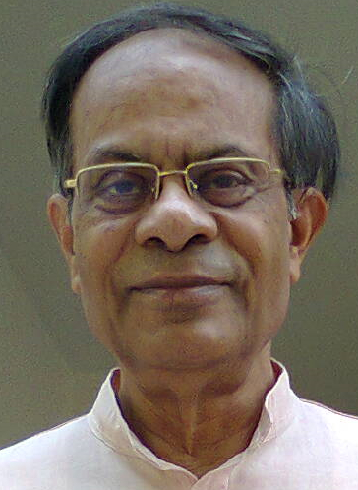
\includegraphics{src/Figures/authors/Rajendra.jpeg}} &

\centerline{\large\bf Rajendra K. Bera}

\bigskip

Dr. Rajendra K. Bera is the Chief Mentor at Acadinnet and a former honorary professor at the International Institute of Information Technology, Bangalore where he taught two courses: quantum computing, and intellectual property rights. In November 2005 he retired as the head of the R\&D group of IBM Software Labs, India. He was with IBM during 1995-2005. Earlier he was a research scientist with the National Aerospace Laboratories, Bangalore (1971-1995); a visiting assistant professor of aerospace, mechanical, and nuclear engineering, University of Oklahoma, USA (1979-1980); and a visiting faculty of aerospace engineering at the Indian Institute of Technology, Kanpur (1988) where he taught fighter aircraft design.\\
 &\\
\clineB{1-2}{2.5}
\end{tabular}

\vskip 1cm

\begin{figure}[H]
\centering

\includegraphics{src/Figures/AI_powered_society_QR.jpg}

\medskip

{\large\sf Access this article on the Web}
\end{figure}
